In this chapter, the process of designing the front-end sampling card is described.
Designing a \gls{pcb} is a two step process: circuit design and layout design.
In this thesis, the software used to cover both of these steps is PADS xDx Designer (for schematic capture) and PADS Layout/Router (for \gls{pcb} layout design) from Mentor Graphics (subsidiary of Siemens).

\section{Schematics}
Without knowing which components are needed and how they are interconnected, it is impossible to manufacture any board, no matter how high or low the level of complexity is.
The main purpose of a schematic is thus to provide a documentation about the necessary components and in which way they should be connected to another.
Furthermore, a schematic provides a starting point for automatic placement and routing, i.e. where the components are placed and how they are connected on the physical \gls{pcb}, which is done with the layout design tool.
During the creation of the schematics, the following points have to be taken into consideration:
%todo a mixture of statements and questions. Choose one
\begin{itemize}
	\item Components: Which components are needed and what are the performance requirement? Especially for high-speed components carefully considering specifications like signal rise and fall times, jitter, skew, etc. is crucial to achieve the overall expected performance.
	\item Connection/Periphery: How many pins are available for peripheral connection? Many components have an interface for programming (e.g. \gls{spi}) which requires several pins. Especially for boards with a lot of components this can quickly become an issue.
	\item Signaling interfaces of the components: Additional circuitry might be needed for interfacing between two different components. Some signaling interfaces, like \gls{lvds}, require a specific voltage level, which might result in the need of voltage level translators.
	\item Common mode voltage: Keep in mind the different common mode voltages at input/output pins of different components and placing decoupling capacitors if needed.
	\item Filtering: Consider placing additional filtering for power supplies, as well as recommended filters from manufacturers of the components. 
	\item Power Supply: Choose suitable power supplies/voltage regulators. How many of them are needed?
	\item Size and Packaging: Packaging of the components. Obviously the size matters, as space on the board is limited. But package also introduces additional capacitance/inductance, which can be a problem for precise filtering circuits. 
	\item Power dissipation: Components, especially voltage regulators, might need coolers. This might not pose any problems for components which are located on the top side of the board. However, components on the bottom side might create an issue, if the designed \gls{pcb} should be mounted on another board.
	\item Availability: Check if the components are still available and if they can be delivered in the given project time.
\end{itemize}  
%todo irgendeine überleitung hinschreiben
 
\paragraph{Decoupling techniques}
Probably the most important part in schematics design is proper decoupling of power supplies, as \glspl{ic} require a stable voltage on the power supply pin for optimal performance.
Any ripple\footnote{\textit{Ripple} is the \gls{ac}-voltage superimposed on an otherwise \gls{dc}-voltage.} or noise can substantially degrade the performance of the \glspl{ic}, i.e. by decreasing the noise margin.
\textit{Noise margin} defines the difference between the useful signal and noise. 
A sufficient noise margin is necessary to guarantee that the output signal will still be correctly interpreted, even if some noise is added to the signal.
Usually, manufacturers give information about proper decoupling circuits for their component in the data sheet.
If this is not the case, there are basic rules of thumb which can be followed to ensure good decoupling. \cite{decouple}

Basically, two types of voltage variations on the power supply pin can be distinguished: low frequency and high frequency variation.
Low frequency variation occurs for example due to devices (or parts of them) being enabled/disabled or in the event of data traffic or data processing.
The current draw during these occurrences can not be compensated immediately by the voltage regulator providing the supply voltage, which leads to drops in the voltage levels.
Time frames of this noise vary in the range of milliseconds up to days.
High frequency variation results from switching events in the device, occurring in the range of the clock frequency and the corresponding harmonics up to about \SI{5}{\giga \hertz}.
Spikes due to \gls{emi} are also a source of high frequency variation and need to be compensated for. \cite{xilDecouple} 

Ideally, one capacitor, which acts as a low-pass filter, should be enough to mitigate these variations.
A real capacitor however has parasitics and thus can in general not be modeled by a ``pure'' capacitive behavior, especially for high-frequency applications. %todo define parasitics
Additional resistances and inductance need to be considered \cite{decouple}:
\begin{itemize}
	\item A parallel resistance $R_P$, which shunts the nominal capacitance ($C$), representing insulation resistance or leakage.
	\item A series resistance $R_S$, or \gls{esr}, which represents the plates and the leads of the capcitor.
	\item A series inductance $L_S$, or \gls{esl}, that models the inductance of the plates and leads of the capacitor.
	\item A parallel resistance and capacitance, $R_D$ and $R_C$, which model the effect called dielectric absorption. This denotes the phenomenon, that a capacitor which has been charged for a long time, doesn't fully discharge when briefly discharged. Dielectric absorption can be detrimental for high-precision use-cases, for power supply decoupling this effect doesn't have to be considered.
\end{itemize}
Considering all these effects leads to the equivalent circuit shown in \autoref{fig:real_cap}.
It can be seen that this forms a RLC circuit, meaning the capacitor will not have the ideal behavior over all frequency range. In fact, a real capacitor shows an impedance response as seen in \autoref{fig:esl_esr}, which resembles one of a band stop, rather than a low pass.
Typical capacitive behavior is seen in region (I).
Region (II) shows the influence of the \gls{esr}, which is why there is a residual impedance at the lowest point.
Region (III) showcases the effect of the \gls{esl}. 
To extend the capacitive behavior over a wider frequency range, at least two capacitors are placed.

\tikzexternaldisable
\begin{figure}[tbh]
	\centering
	\includegraphics[width = .7\textwidth]{chap/04-work/img/real_cap.tikz}
	\caption[Capacitor equivalent circuit]{Equivalent circuit of a real capacitance (redrawn from \cite{decouple})}
	\label{fig:real_cap}
\end{figure}
\tikzexternalenable
\begin{figure}[tbh]
	\centering
	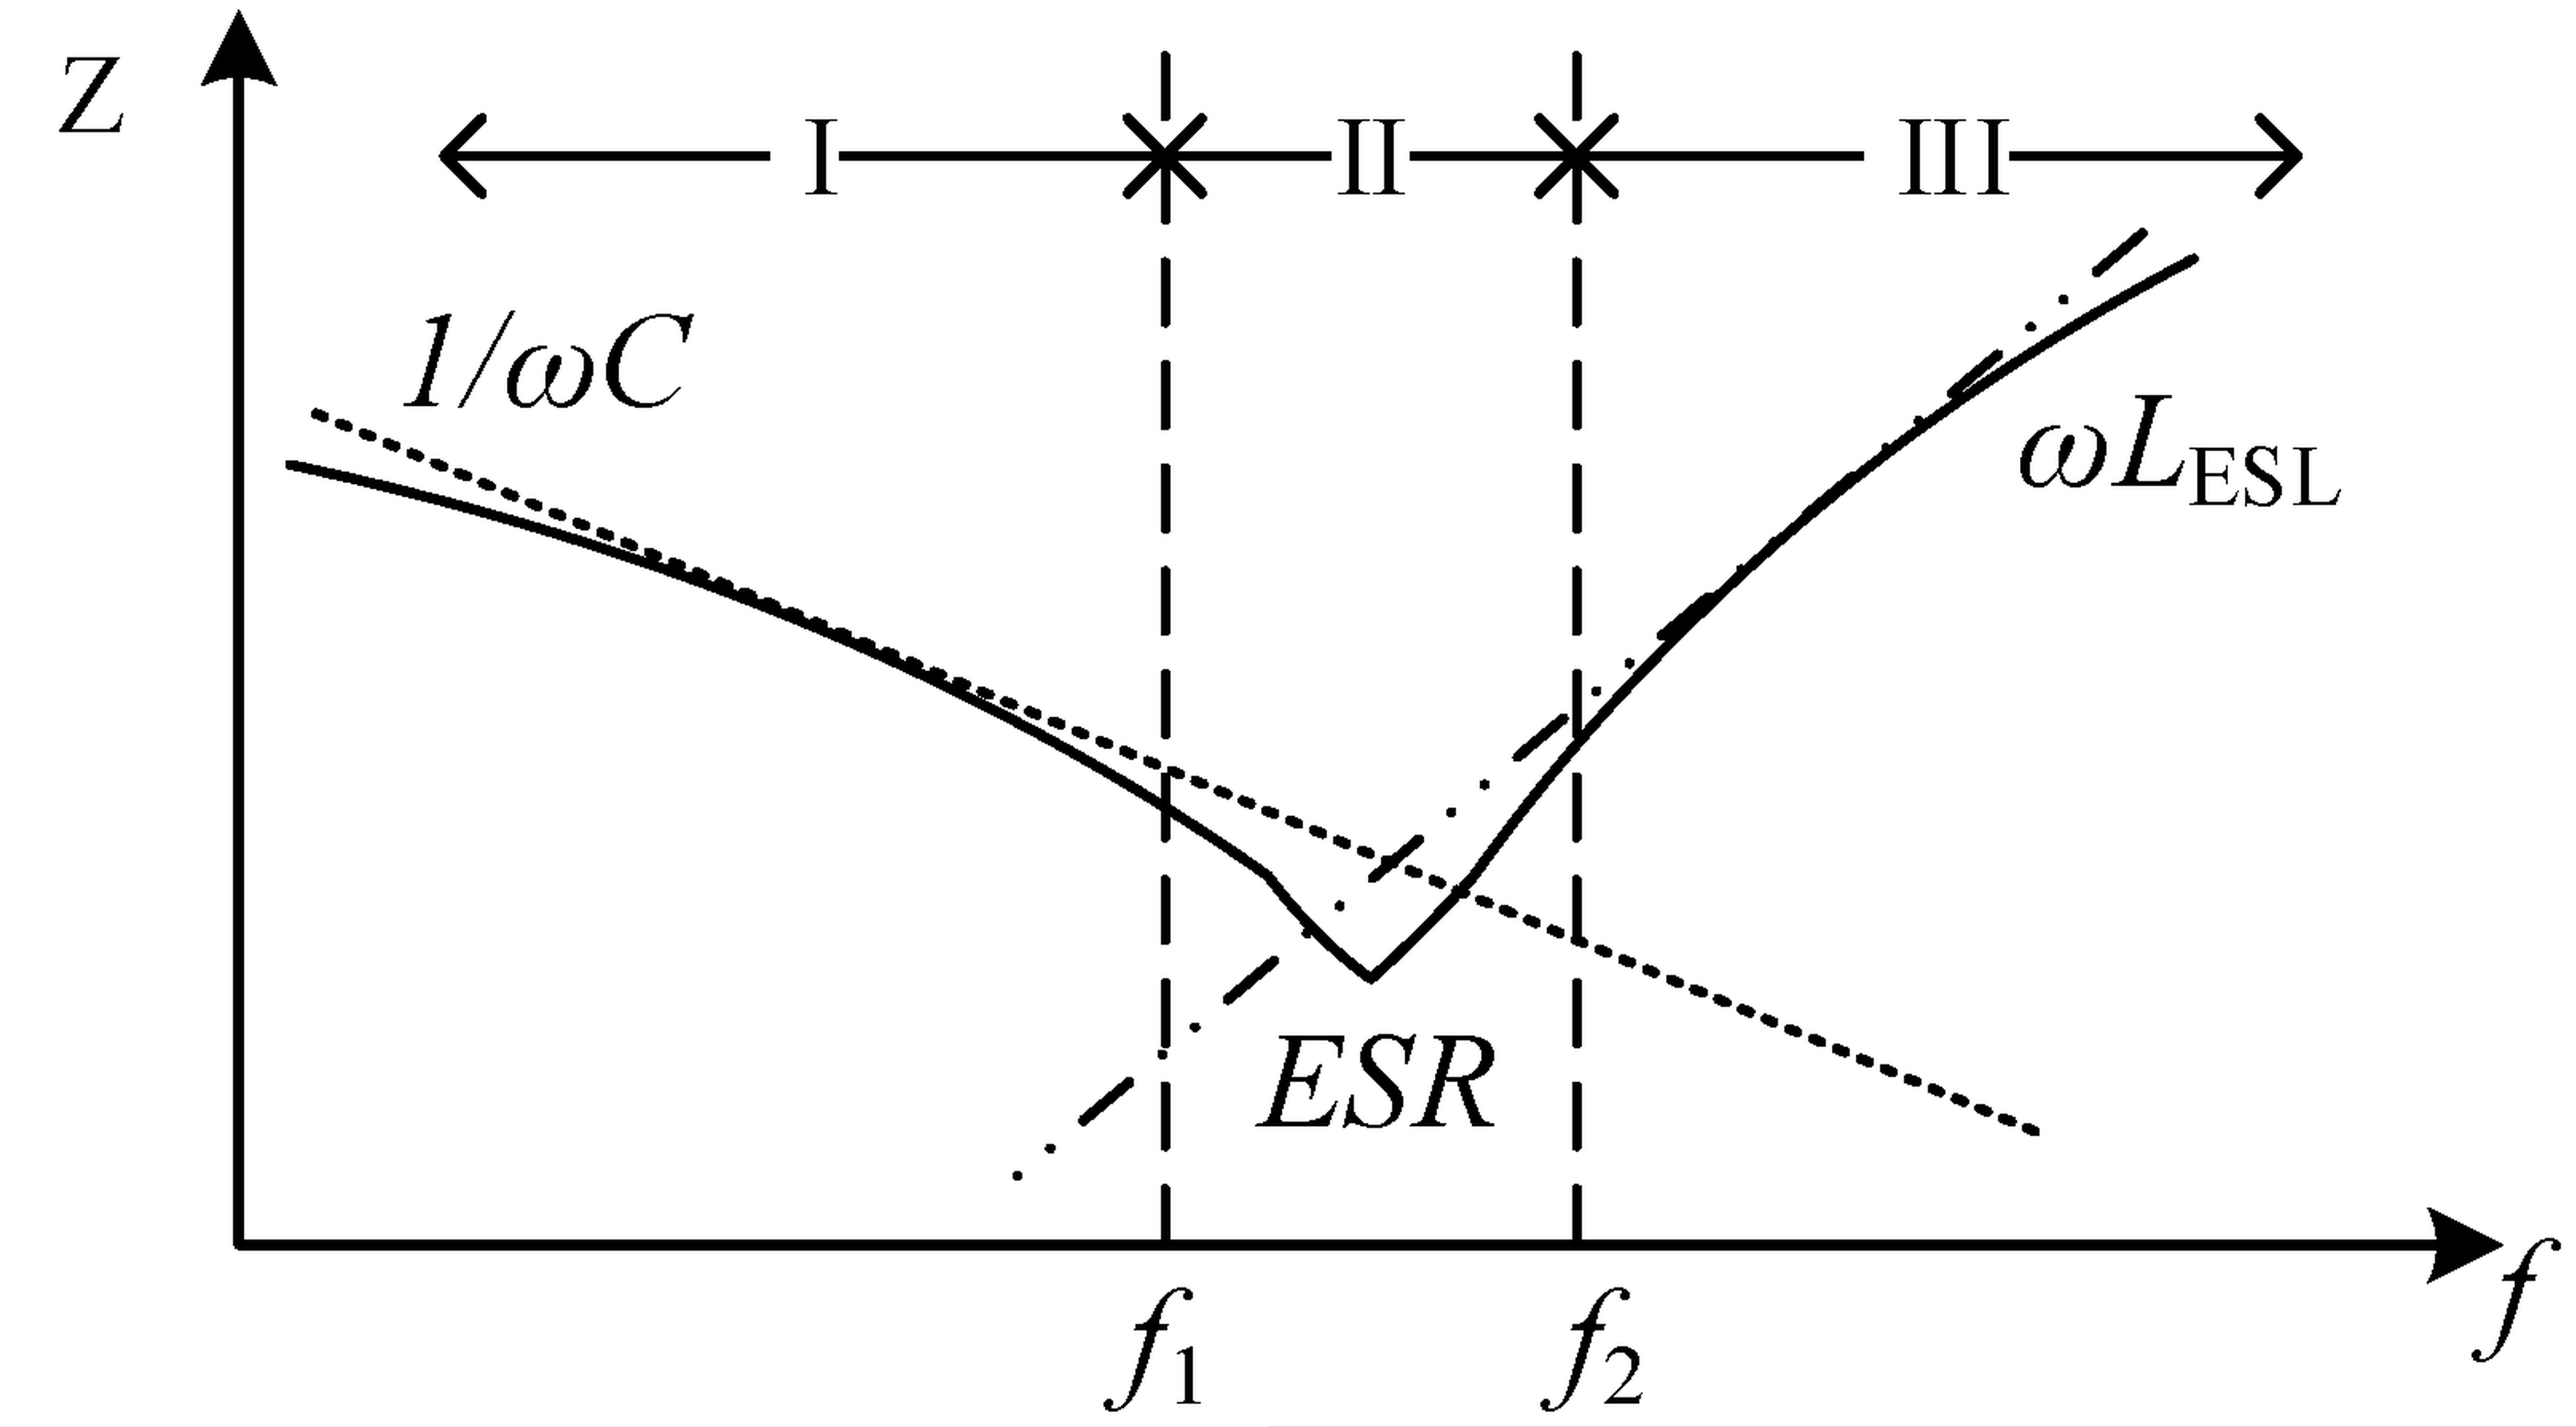
\includegraphics[width = \textwidth]{chap/04-work/img/esl_esr}
	\caption[Impedance response of a real capacitor]{Qualitative impedance response of a real capacitance \cite{Dang2020}}
	\label{fig:esl_esr}
\end{figure}


To deal with the low frequency variation, a large capacitor (typical values: 10 - \SI{100}{\micro \farad}) is placed next to the chip, not more than \SI{5}{\centi \metre} ($\approx$ 2 inch.) away.
The role of this capacitor is to be a charge supply for the instantaneous needs of the device, i.e. "taking the role" of the voltage regulator until the latter can adjust to the changed current draw. \cite{decouple}
%todo maybe <<...keeping a constant voltage level until the slower control loop of the voltage regulator can compensate for...>>

A small capacitor (typical values: 0.01 - \SI{0.1}{\micro \farad}), placed as close as possible to the power pins of the component.
This capacitor should bypass the high frequency variation on the power supply line. \cite{decouple}

All capacitors should be connected through vias\footnote{See \autoref{ssec:pcb_structs}} or short traces to a large area, low impedance ground plane\footnote{See \autoref{ssec:pcb_structs}}. %todo via? large area?
This way the inductance due to connection traces is minimized. \cite{decouple}

An optional ferrite bead in series with the supply pin keeps external high frequency from the device and the internally generated noise from the rest of the board. \cite{decouple}

\paragraph{Separating Analog and Digital Ground}
TODO


%todo maybe some more theory, e.g. that real capacitor has resistive and inductive components due to packaging, connection and dielectric. doesn't behave like a capacitor at high frequencies -> several capacitors needed to ensure capacitive behaviour at high frequencies

\subsection{Connectors}\label{sec:connectors}
The number and type of connectors is primarily defined by the read-out card, on which the sampling board is mounted.
The different connector types serve different purposes, which can be organized into three categories.

\paragraph{Digital Control Signals}
For digital control signals (i.e. \gls{spi}, enable signals, \ldots) and clocking a VITA 57.4 FMC+ connector from \textit{SAMTEC} is used (see \autoref{fig:fmcp}). 

\gls{fmc} is a standard defined by \gls{vita} to provide a standard mezzanine card\footnote{A \gls{pcb} which is plugged on a plug-in board. \cite{mezzanine}} form factor, connectors, and modular interface to a \gls{fpga} located on a base board (carrier card). \cite{Seelam2009}
The \gls{fmc}+ standard extends the pin count and throughput of the present high-speed interfaces. 

This connector provides 560 pins arranged in a $14\times40$ array, 80 of which are additional high-speed interfaces, located on either side of the connector (therefore this connector type is also called \gls{hspce} connector, as opposed to the HSPC connector which doesn't have additional rows).
For user-defined purpose 160 pins are available. 
They can be used as single-ended or differential pins.
Clocking capable pins can be used to propagate clock signals from the mezzanine to the carrier board. 

Furthermore, the connector provides pins for power supply from carrier board to mezzanine card \cite{fmc}:
\begin{itemize}
	\item VADJ: Voltage adjustable from 0 to \SI{3.3}{\volt} (max. \SI{4}{\ampere}, max. \SI{1000}{\micro \farad} capacitive load) 
	\item \SI{3.3}{\volt} (max. \SI{3}{\ampere}, max. \SI{1000}{\micro \farad} capacitive load)
	\item \SI{12}{\volt} (max. \SI{1}{\ampere}, max. \SI{1000}{\micro \farad} capacitive load)
\end{itemize}
%todo to table?

An assembly drawing of the connectors is shown in \autoref{fig:fmcp}.

\begin{figure}[tbh]
	\centering
	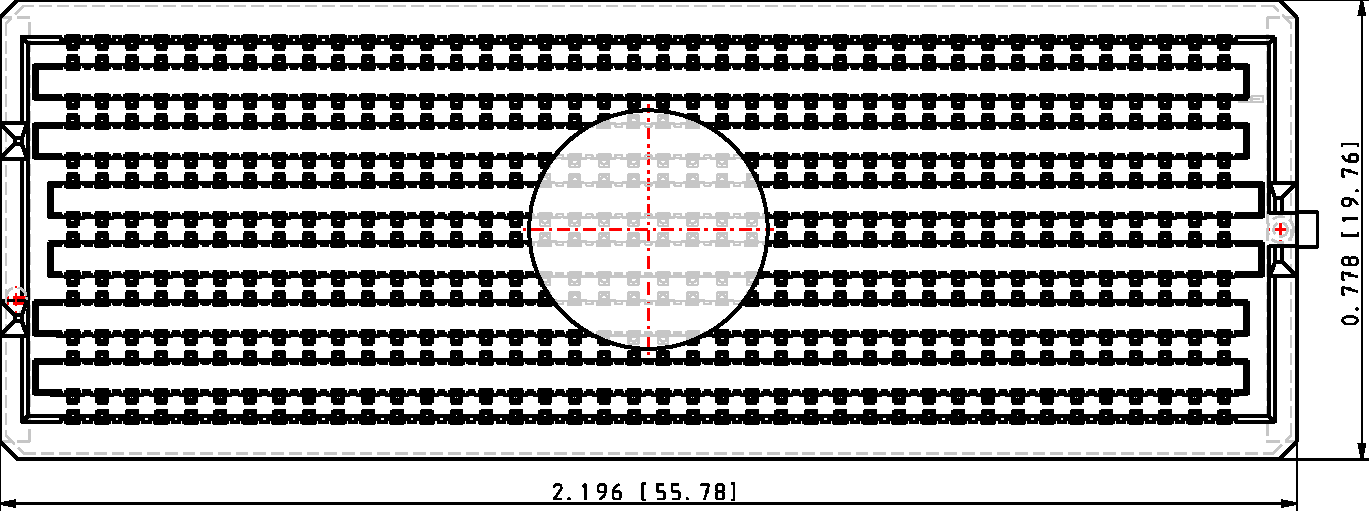
\includegraphics[width = 0.7\textwidth]{chap/04-work/img/fmcp.pdf}
	\caption[Rendering of FMC+ connector]{Part drawing of FMC+ connector \cite{fmcpic}}
	\label{fig:fmcp}
\end{figure}

\paragraph{Analog Signals}
The signal from the detector is provided to the \glspl{tha} through \gls{sma}\footnote{Coaxial \gls{rf} connector} \gls{rf} connectors from \textit{molex}, which are mounted at the edge of the board.
\autoref{fig:sma} shows a 3D model of this connector type. 

\begin{figure}[tbh]
	\centering
	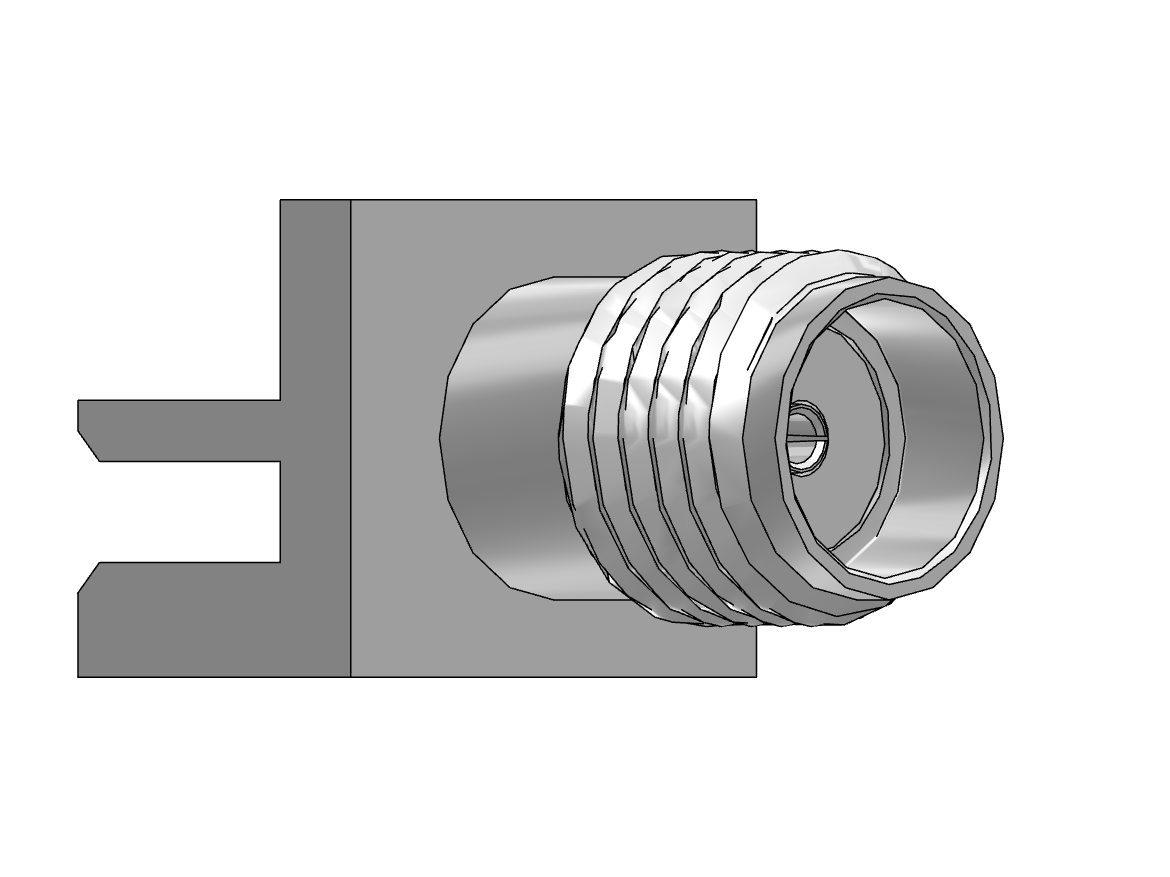
\includegraphics[width = 0.5\textwidth]{chap/04-work/img/sma}
	\caption[Edge-Mount RF SMA connector]{3D model of the edge-mount \gls{rf} \gls{sma} connector from \textit{molex} \cite{molex}}
	\label{fig:sma}
\end{figure}

On the read-out board two RFMC 2.0 (\gls{rf} Mezzanine Card) interface connectors are provided.
The connectors used are \gls{lpaf} connectors from \textit{SAMTEC} with 400 pins arranged in a $8\times50$ array.
One is dedicated for transmitting signals from the mezzanine card to the on-board \glspl{adc}.
The other provides the analog output from the on-board \glspl{dac}\footnote{A \gls{dac} translates digital values into an analog signal.} to the mezzanine card.
On the sampling board, the male counterpart of the connectors, \gls{lpam}, is used (see \autoref{fig:lpam1}).

\begin{figure}[tbh]
	\centering
	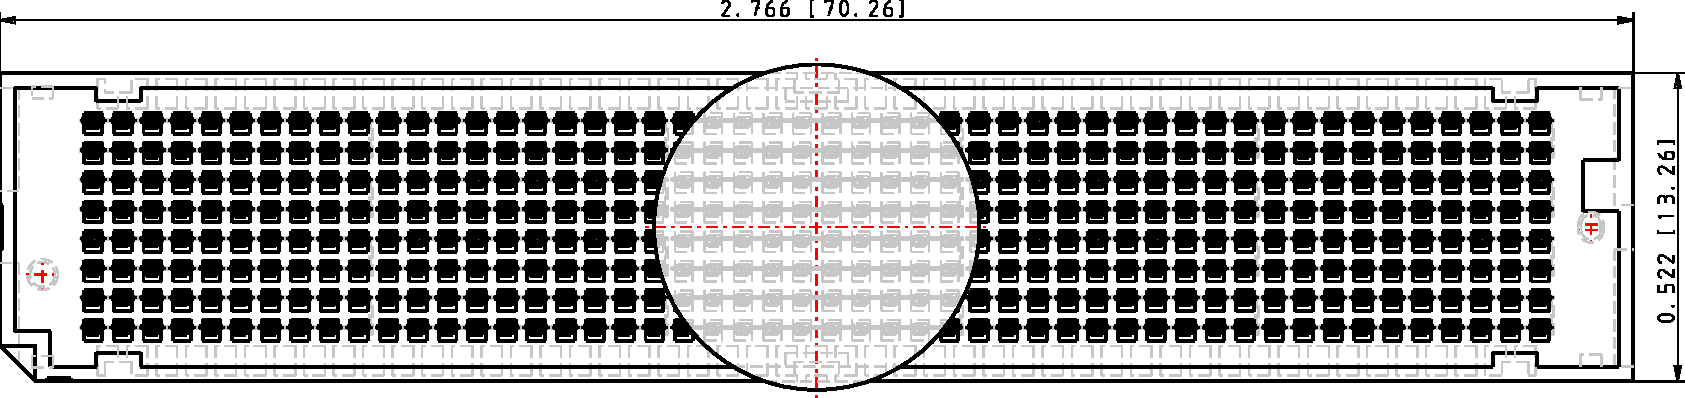
\includegraphics[width = \textwidth]{chap/04-work/img/lpam_50_top.pdf}
	\caption[LPAM $8\times50$ connector]{Part drawing of a LPAM $8\times50$ connector}
	\label{fig:lpam1}
\end{figure}


\paragraph{Clock Signals}
The clock signals from the \glspl{pll} on the sampling board are propagated in different ways.
The reference clock for the \gls{fpga} is propagated through the \gls{fmc}+ connector.
Clocking for the \glspl{adc} and the \glspl{dac} is provided through a $6\times20$ \gls{lpam} connector (see \autoref{fig:lpam2}).




\begin{figure}[tbh]
	\centering
	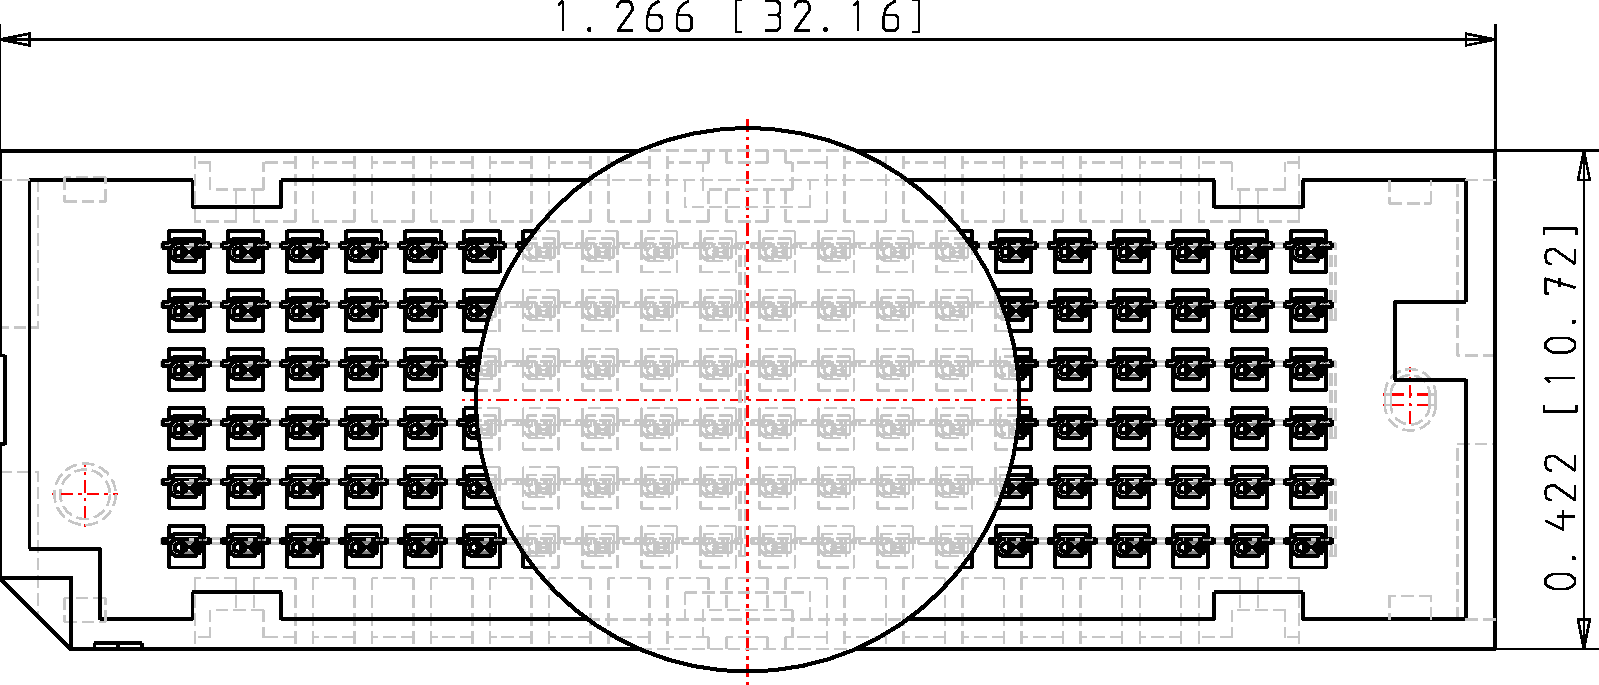
\includegraphics[width = 0.7\textwidth]{chap/04-work/img/lpam_20.pdf}
	\caption[LPAM $6\times20$ connector]{Part drawing of LPAM $6\times20$ connector}
	\label{fig:lpam2}
\end{figure}

%todo other pictures of connectors? maybe photos/renderings are better?



\subsection{Sampling-Channel}
The sampling channel consists of the \gls{tha}, which is driven by a delay chip. 

\paragraph{Track-And-Hold-Amplifier}
The \gls{tha} used is the same as in \gls{kapture}. The component was chosen such that jitter lies in the range of hundreds of femtoseconds. \cite{caselle2013}
According to the data sheet \cite{hmc5640}, the component shows the characteristics shown in \autoref{tab:hmc5640}.
\begin{table}[tbh]
	\caption[HMC5640 Characteristics]{Specifications of the HMC5640 \gls{tha}}
	\label{tab:hmc5640}
	\begin{minipage}{\textwidth}
		\centering
		\begin{tabularx}{\textwidth}{Xcccc}
			\toprule
			\textbf{Parameter} & \textbf{Min} & \textbf{Typ.} & \textbf{Max} & \textbf{Unit}\\
			\midrule
			\textbf{Analog Inputs} &&&& \\
			Differential \gls{fs} Range & & 1 & & Vpp\footnote{Volt peak-to-peak}\\
			Common mode voltage & -0.1 & 0 & 0.1 & V\\[0.3cm]
			\textbf{Clock Inputs} &&&&\\
			DC Differential High Voltage (Track Mode) & 20 & 40 & 2000 & mV\\
			DC Differential Low Voltage (Hold Mode) & -2000 & -40 & -20 & mV\\
			Common mode voltage & -0.5 & 0 & 0.5 & V\\[0.3cm]
			\textbf{Analog Outputs} &&&&\\
			Differential \gls{fs} Range &  & 1 && Vpp\\
			Common mode voltage & & 0 & & V\\[0.3cm]
			\textbf{Track-to-Hold/Hold-to-Track Switching} &&&&\\
			Aperture Delay & & -6 &  & ps\\
			Random Aperture Jitter (\gls{fs}, \SI{1}{\giga \hertz}) & & < 70 & & fs\\
			Settling time\footnote{\textit{Settling time} is the interval between the internal track-hold transition and the time when the output signal is settled within the specified value.} (to \SI{1}{\milli \volt}) &	&  116 & & ps \\
			\bottomrule
		\end{tabularx}
	\end{minipage}
\end{table}

As the analog input to the \gls{tha} is single-ended, a \SI{50}{\ohm} termination on the unused input pin has been added, as recommended in the data sheet.\cite{hmc5640}
%todo 	explain transmission lines and termination?

At the power pins, decoupling capacitors and a ferrite bead  were placed. The \gls{tha} is a crucial component, as it samples the detector signal, therefore any possible noise should be reduced to a minimum.

\begin{figure}[tbh]
	\centering
	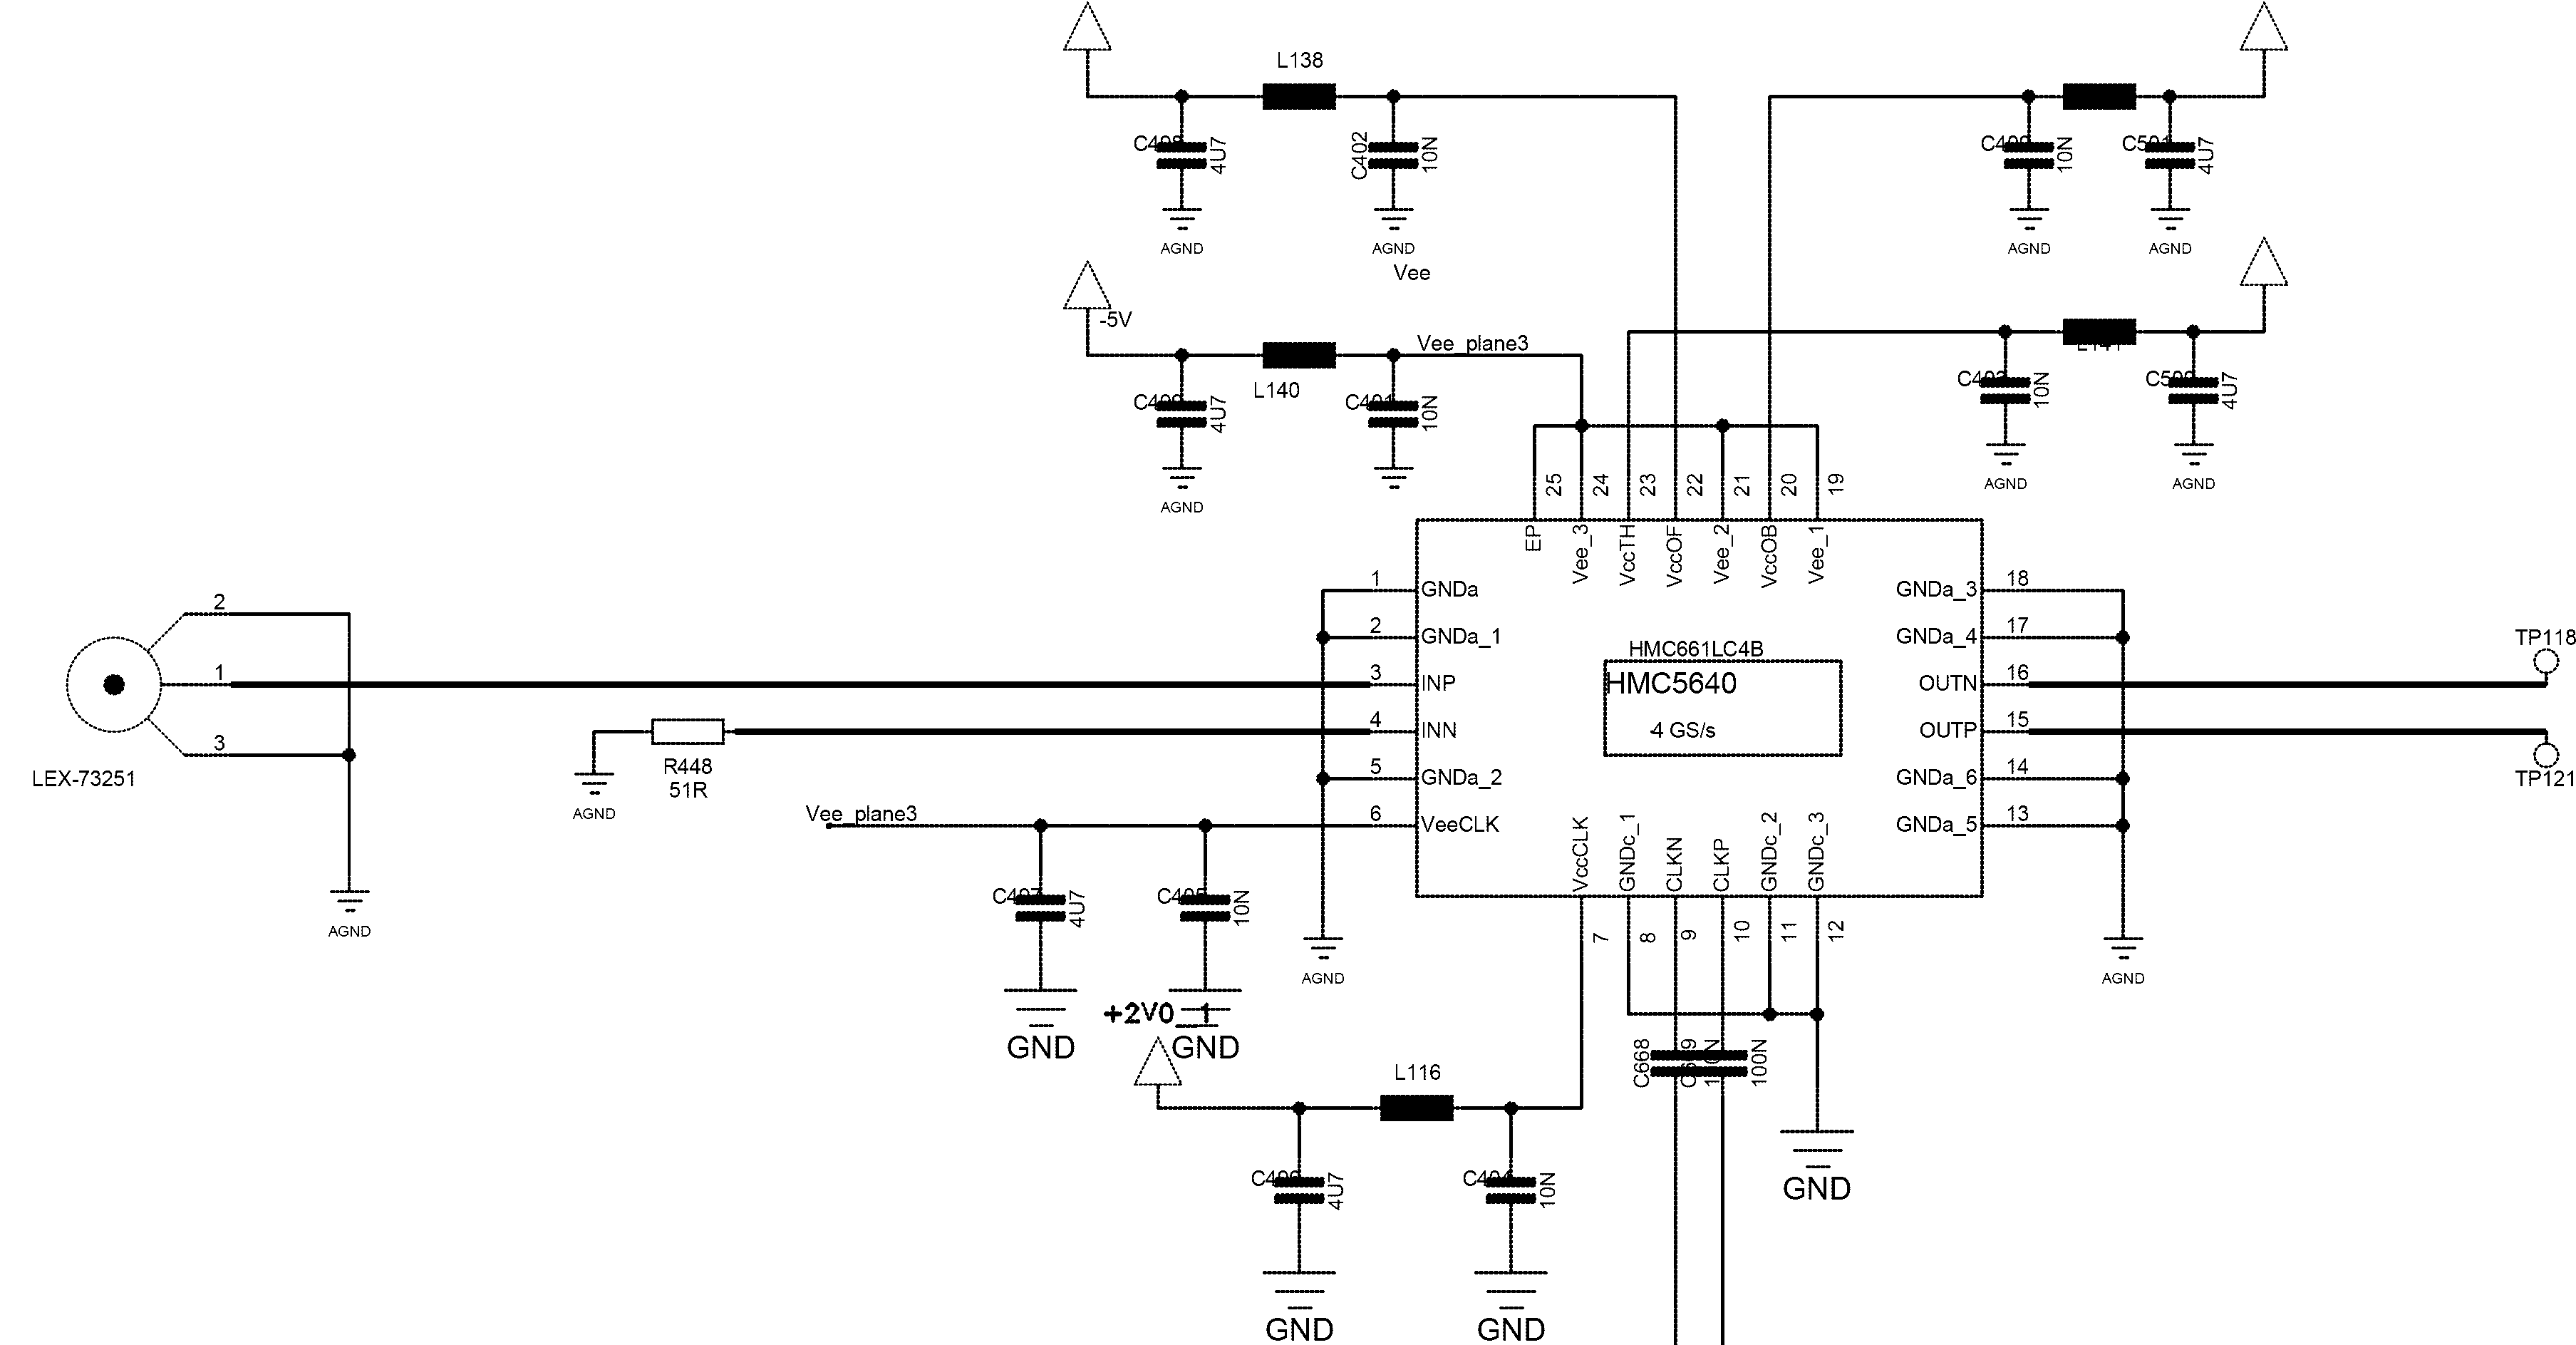
\includegraphics[width = \textwidth]{chap/04-work/img/hmc5640}
	\caption[HMC5640 THA schematic]{HMC5640 \gls{tha} schematic}
	\label{fig:hmc5640}
\end{figure}
%todo better picture/somehow improve this BS
%todo maybe only a pic of the component itself


\paragraph{Delay Chip}
The delay chip is used to create a delay in the clocking signal, which then goes to the \gls{tha} chip. For the selection of the delay chip, the most important characteristic, apart from jitter, is the delay step size and delay range. 

The delay step size must be small enough, such that the \gls{adc} interleaving technique \autoref{sssec:time-interleaving} can be implemented.
The \glspl{adc} on the read-out card sample at a maximal sample rate of \SI{2.5}{\giga \sample \per \second}, meaning during the time
\begin{equation}
	t_s = \frac{1}{\SI{2.5}{\giga \sample \per \second}} = \SI{400}{\pico \second}
\end{equation}
all 16 \glspl{adc} have to be clocked one time.
This means, a delay step can not be greater than $\nicefrac{\SI{400}{\pico\second}}{16} = \SI{25}{\pico\second}$.

With the HMC856 programmable delay chip from \textit{Analog Devices}, which is also used for the \gls{kapture} sampling, a minimal step size of \SI{3}{\pico\second} \cite{hmc856} is possible.
However, one drawback is the maximal delay range of \SI{100}{\pico\second}.
Considering a signal, which is stretched over several nanoseconds, this range limits the possibility to freely chose the resulting timing resolution.
The major problem is the programming interface of the chip, which consists of five differential \gls{cml} inputs.
This means, one chip already takes up 10 pins.
For in total 16 necessary delay chips, this results in 160 pins occupied only by the delay chips.
This occupies all pins of the \gls{fmc}+ connector (see \autoref{sec:connectors}) available for the user. 

A better candidate is the dual channel programmable delay chip NB6L295 from \textit{ON Semiconductor}.
This chip provides two programmable delay channels, therefore effectively reducing the chip count by half.
With a delay step size of \SI{11}{\pico\second} it is still suitable for the targeted interleaving method, covering a total delay range from \SI{3.2}{\nano\second} to \SI{8.8}{\nano\second} per delay channel.
The chip is programmed via \gls{sdi}, which only requires 4 pins (enable pin, data pin, clock pin, load pin). %todo maybe explain the pins more, don't know
Thus, the total number of digital control pins used by the delay chips is $4\cdot8 = 32$, which is a significant reduction compared to the 160 control pins needed by the HMC856.
\begin{figure}[tbh]
	\centering
	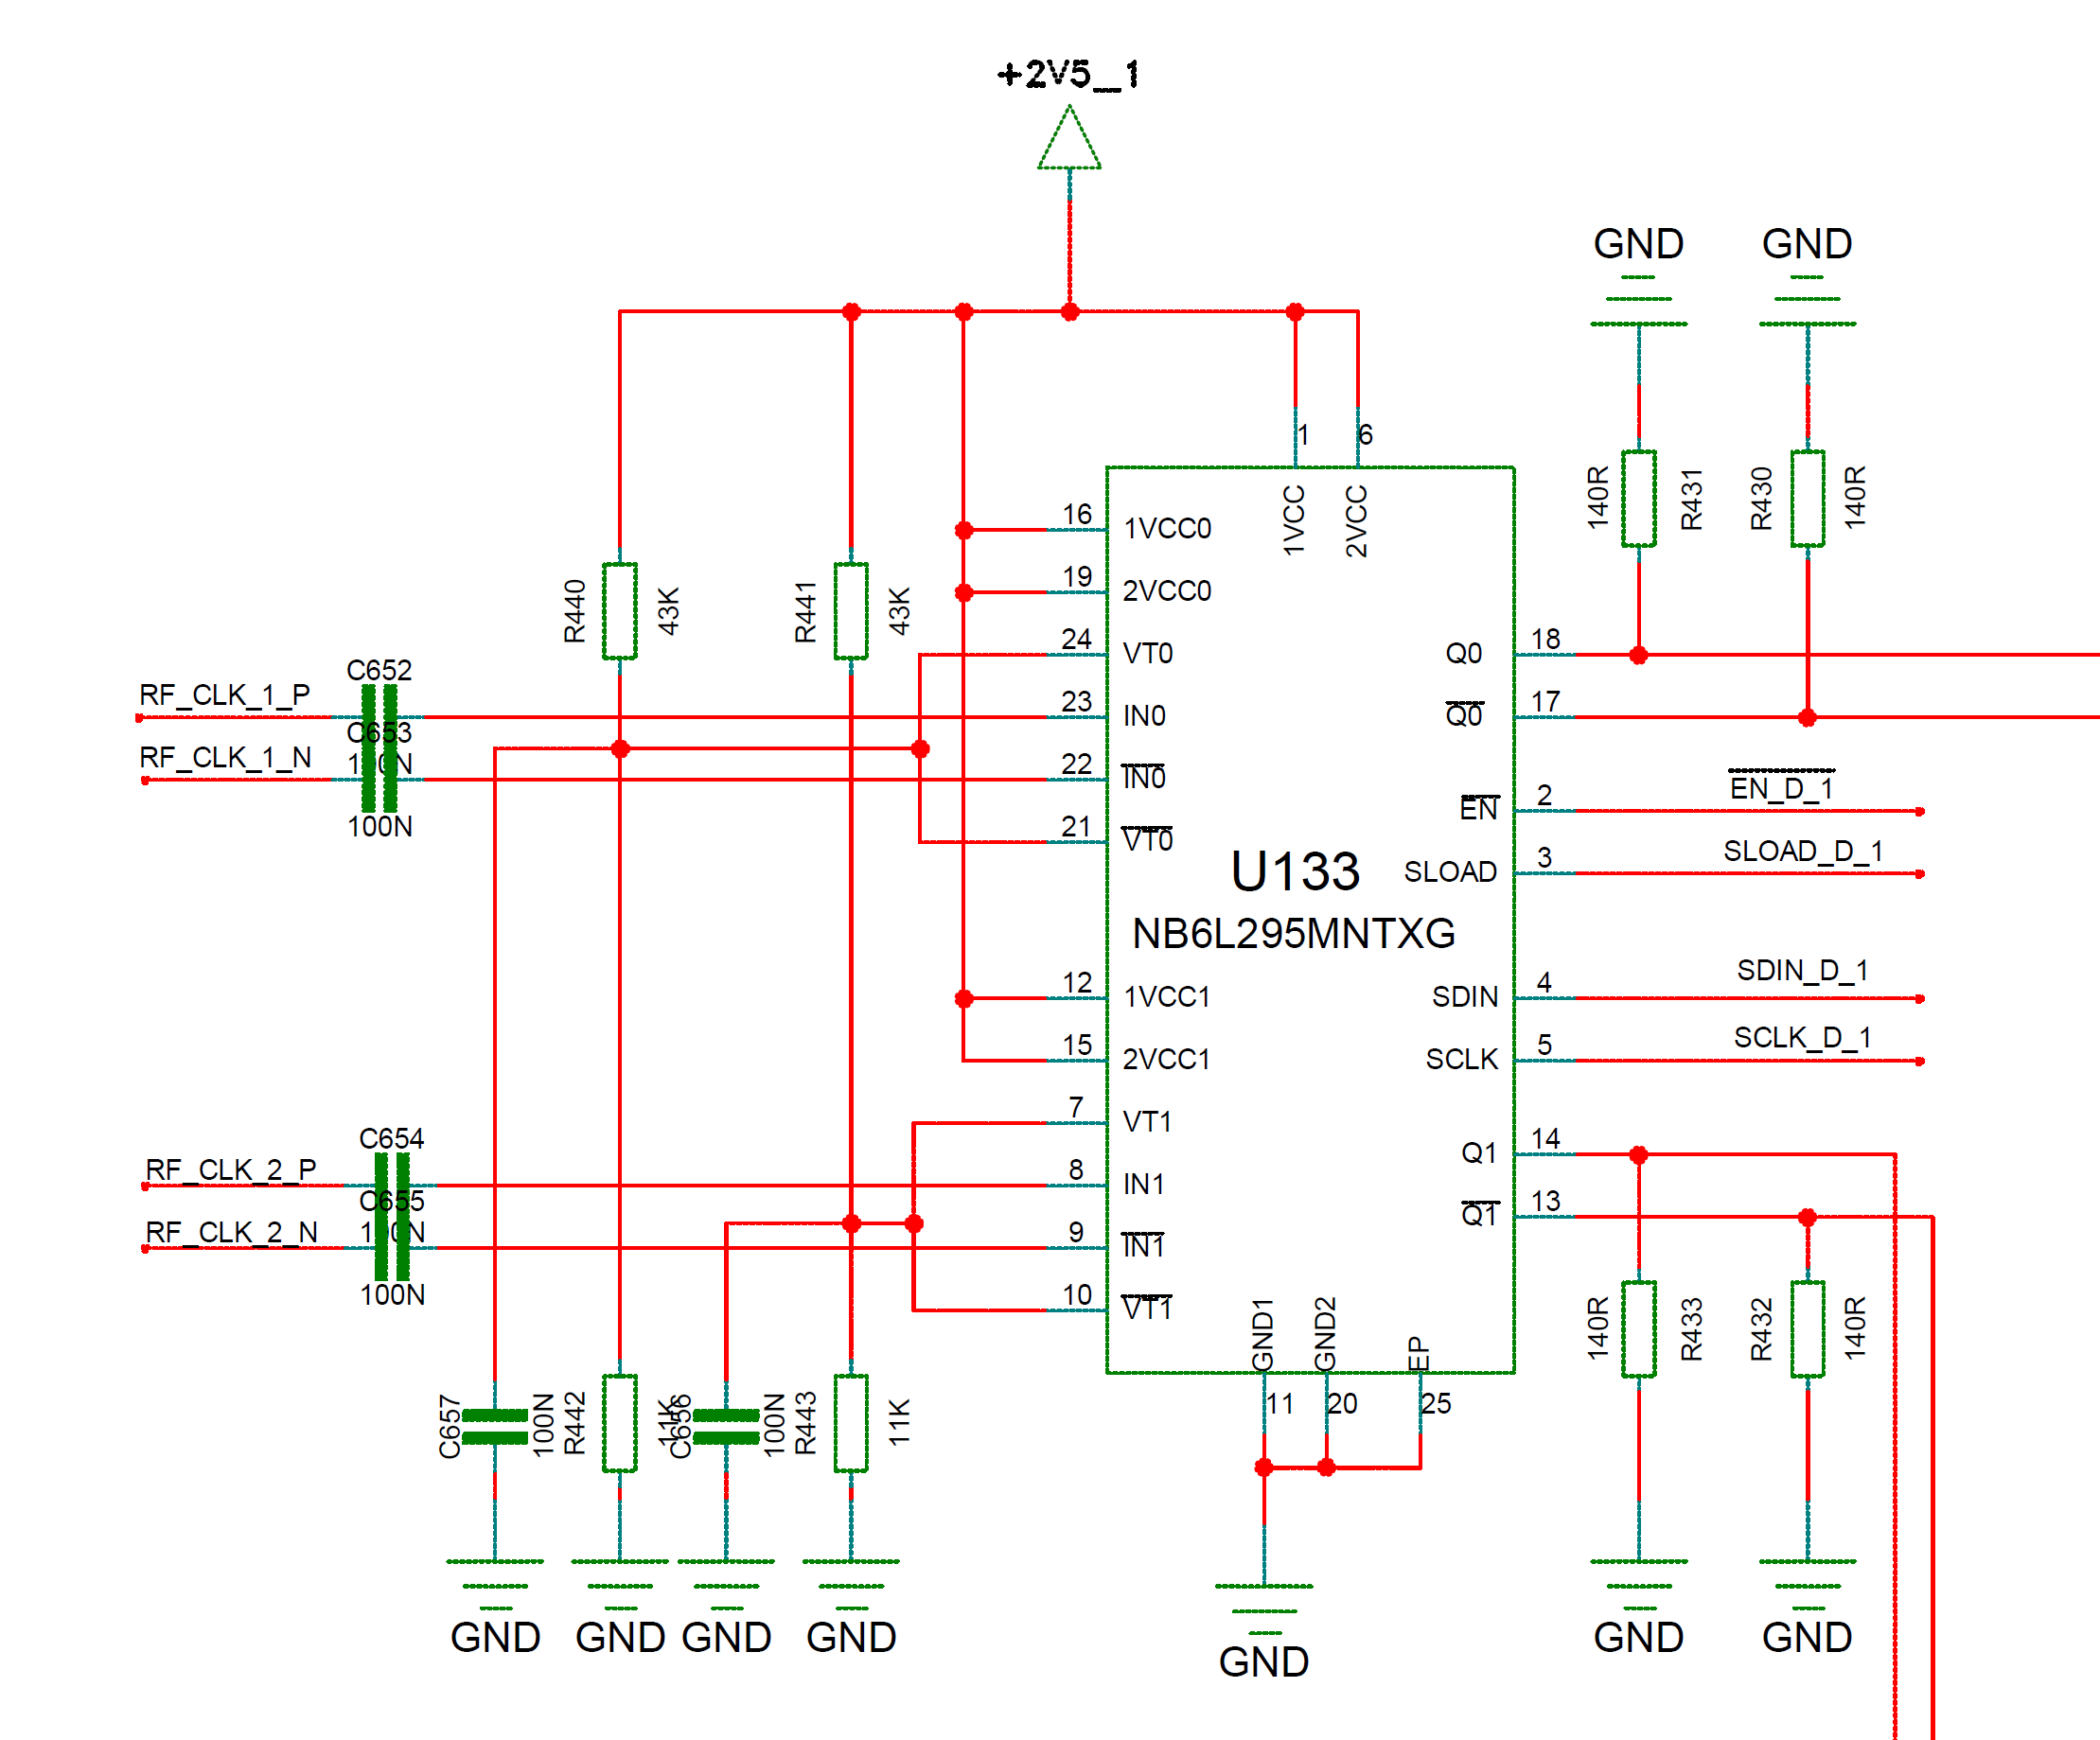
\includegraphics[width = \textwidth]{chap/04-work/img/delay_chip}
	\caption[NB6L295 delay chip schematic]{NB6L295 schematic}
	\label{fig:nb6l295}
\end{figure}

\paragraph{Outputs}
The output of the delay chip is using a \gls{lvpecl} signaling interface, which is based on an open-emitter topology (see \autoref{fig:lvpecl}).
This requires a path to \gls{dc}, which is achieved by adding \SI{140}{\ohm} resistors.

\begin{figure}[tbh]
	\centering
	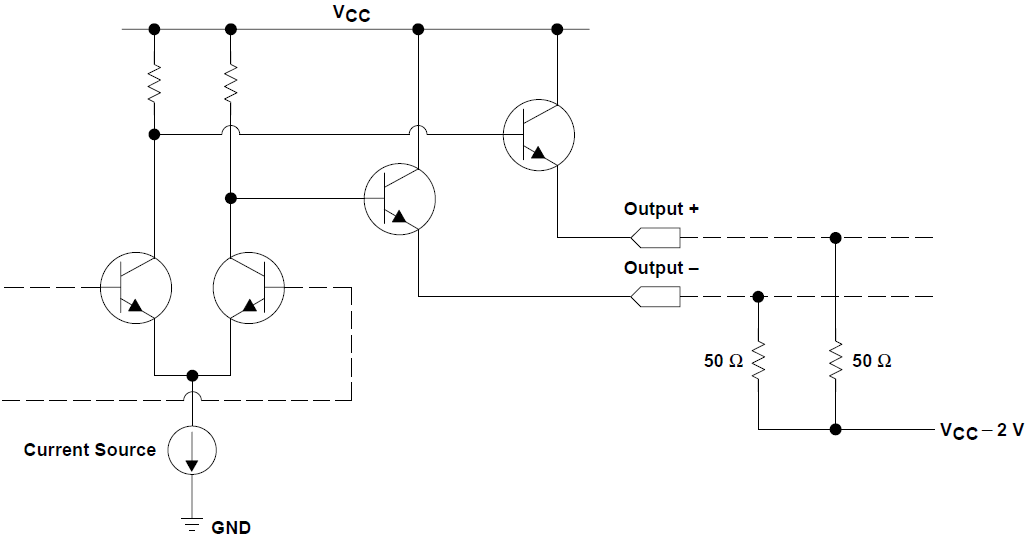
\includegraphics[width = \textwidth]{chap/04-work/img/lvpecl}
	\caption[LVPECL driver topology]{LVPECL driver topology. Left side shows the emitter-follower based driver. On the right, an example biasing with resistors is shown. \cite{lvpecl}}
	\label{fig:lvpecl}
\end{figure}
%todo to tikz

As the output will be connected to the \gls{tha}, it is necessary to check the compatibility of the maximum amplitude and common-mode.
According to the data sheet \cite{NB6L295}, the voltage level of the output can vary between  $V_\text{cc} - \SI{1825}{\milli\volt}$ and $V_\text{cc} - \SI{825}{\milli\volt}$ (see \autoref{tab:nb6l295}).
Maximal voltage amplitude acceptable by the \gls{tha} inputs is \SI{2000}{\milli\volt} (see \autoref{tab:hmc5640}).
When using a supply voltage of $V_\text{cc} = \SI{3.3}{\volt}$, provided e.g. by the read-out card through the \gls{fmc}+ connector, this leads to a maximum output level of \SI{2475}{\milli\volt}.
This exceeds the limit given by the \gls{tha}.
Therefore, for $V_\text{cc}$ a smaller voltage should be considered.
In this design a voltage of $V_\text{cc} = \SI{2.5}{\volt}$ is chosen, which guarantees that the amplitude falls within the range \SIrange{675}{1675}{\milli\volt}.

The common mode voltage $V_{\text{CM}}$ is calculated as %todo why?
\begin{equation}
	V_{\text{CM}} = \frac{\SI{675}{\milli \volt} + \SI{1675}{\milli \volt}}{2} = \SI{1175}{\milli \volt}.
\end{equation}

This is higher than the maximal input common mode voltage of $\SI{0.1}{\volt}$ of the \gls{tha}(see \autoref{tab:hmc5640}).
\gls{ac} coupling is therefore necessary in this case.


\paragraph{Inputs}
When driving the inputs with a \gls{lvpecl} driver (output from the preceding \gls{pll}), the VTx and $\overline{\text{VTx}}$ pins of the delay chip need to be connected to $V_\text{cc} - \SI{2}{\volt}$ (see \autoref{fig:delay_lvpecl}).
In case of $V_\text{cc} = \SI{2.5}{\volt}$, this results in a voltage level of $\SI{0.5}{\volt}$.
To avoid using an additional voltage regulator, this voltage level is achieved by using a resistive voltage divider connected to $V_\text{cc}$.
Choosing the resistor values $\SI{43}{\kilo\ohm}$ and $\SI{11}{\kilo\ohm}$ results in a voltage of
\begin{equation}
	V_\text{cc} \frac{\SI{11}{\kilo\ohm}}{\SI{11}{\kilo\ohm} + \SI{43}{\kilo\ohm}} = \SI{0.5093}{\volt} \approx \SI{0.5}{\volt}
\end{equation}
%todo maybe give the circuit used with R1 and R2 or sth

A \SI{100}{\nano\farad} capacitor is put in parallel for power supply decoupling.

\begin{figure}[tbh]
	\centering
	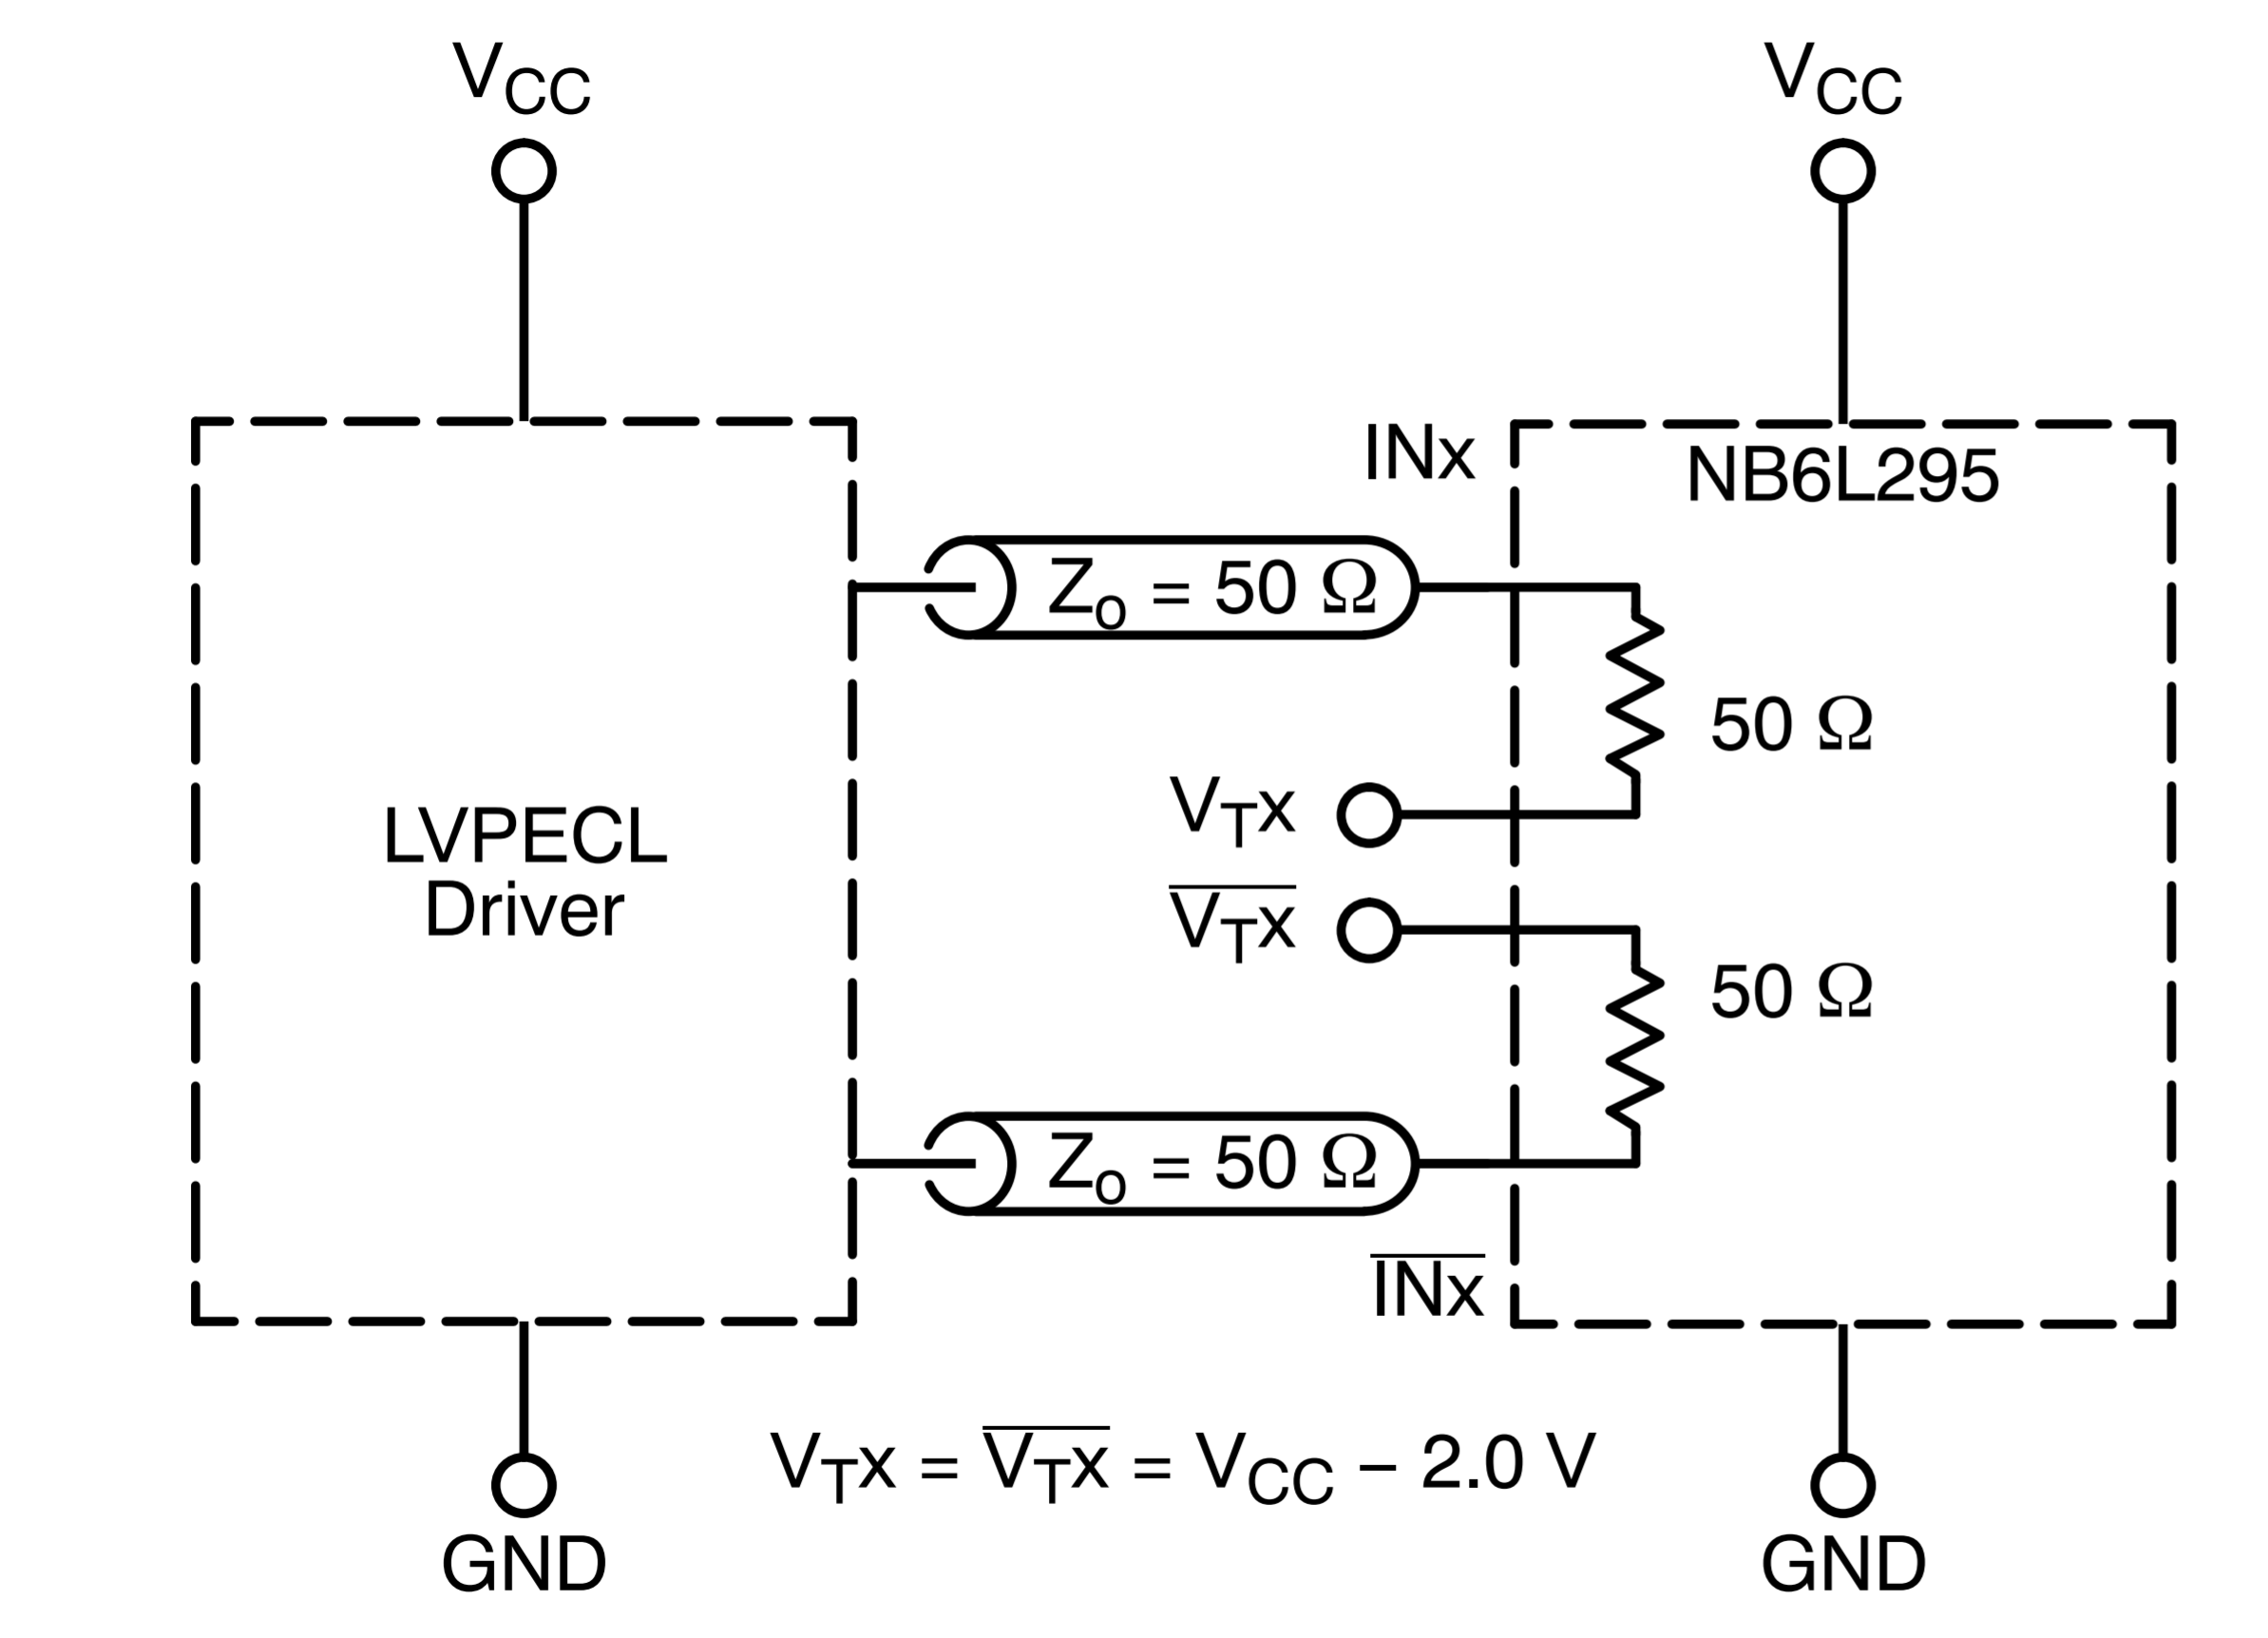
\includegraphics[width = 0.7\textwidth]{chap/04-work/img/delay_lvpecl}
	\caption[NB6L295 Delay Chip Schematic]{LVPECL recommendations for NB6L295 \cite{NB6L295}}
	\label{fig:delay_lvpecl}
\end{figure}


\begin{table}[tbh]
	\caption[NB6L295 Characteristics]{Specifications of the NB6L295 delay chip \cite{NB6L295}}
	\label{tab:nb6l295}
	\begin{minipage}{\textwidth}
		\centering
		\begin{tabularx}{\textwidth}{Xcccc}
			\toprule
			\textbf{Parameter} & \textbf{Min} & \textbf{Typ.} & \textbf{Max} & \textbf{Unit}\\
			\midrule
			\textbf{Outputs} &&&& \\
			Output HIGH Voltage & $V_{cc} - 1075$ & $V_{cc} - 950$ & $V_{cc} - 825$ & mV\\
			Output LOW Voltage & $V_{cc} - 1825$ & $V_{cc} - 1725$ & $V_{cc} - 1625$ & mV\\
			Common mode voltage & -0.1 & 0 & 0.1 & V\\[0.3cm]
			\textbf{AC Characteristics} &&&&\\
			Random Clock Jitter \gls{rms}&  & 3 & 10 & ps\\
			Output Rise/Fall Times (@\SI{50}{\mega \hertz}) & 85 & 120 & 170 & ps\\
			Serial Clock Input Frequency (50\% Duty Cycle\footnote{Percentage of the ratio of pulse width and total period of the waveform.}) &  &  & 20 & MHz\\
			Minimum Pulse width SLOAD  & 1 &  &  & ns\\
			\bottomrule
		\end{tabularx}
	\end{minipage}
\end{table}
%todo fix problem with [XSSSSS]
%todo parameters all caps, some capitalized, some not. choose one style


\subsection{Clocking}
TODO:
\begin{itemize}
	\item Brief theory about \gls{pll} -> VCO, Loop Filter, Charge pump, etc.
	\item Maybe some simulation with the PLLatinum Tool (used for calculation of the noise, jitter, etc. over the frequency)
\end{itemize}
Clocking distribution is designed as shown in \autoref{fig:clocking}.
The LMK0480x low-noise clock jitter cleaner \gls{pll} from \textit{Texas Instruments} cleans the incoming reference clock coming from the system (e.g. from \gls{kara}) for high temporal accuracy \cite{caselle2013}.
It is used with an external \gls{vcxo} from \textit{ABRACON}.
The LMK0480x has only 12 outputs, not enough for the 16 \glspl{tha} and additional clocking for \gls{fpga}, \gls{adc} and \gls{dac}, especially considering that the outputs are divided into six groups à two outputs. Outputs in one group have the same configuration (frequency, phase, \ldots), which means that effectively only six different outputs are available.
A low noise clock distribution fan-out buffer, the HMC987LP5E from \textit{Analog Devices} is therefore used for distributing the clock signal to the delay chips.
As one fan-out buffer has eight outputs, two chips are needed to cover all channels.
One output of the \gls{pll} is propagated to the \gls{fmc}+ connector as reference clock for the \gls{fpga}.
Up until this part, this architecture is not different from the one on the \gls{kapture} sampling board. 

\begin{figure}[tbh]
	\centering
	\includegraphics[width = \textwidth]{chap/04-work/img/pll_tsMode}
	\caption{Placeholder}
	\label{fig:clocking}
\end{figure}
%todo clean picture

The maximum output frequency of the LMK0480 is \SI{1536}{\mega \hertz}, not enough to clock the \glspl{adc} at maximum sampling rate (\SI{2.5}{\giga \sample \per \second}). A second \gls{pll} is therefore needed. The read-out card is provided with an \gls{rf} Clock add-on card, which is necessary to generate the high-frequency clocks for the converters. The LMX2594 from \textit{Texas Instruments} provides clocking signal up to \SI{15}{\giga \hertz} and is a fitting candidate. For loop filter calculation, the TI PLLAtinum Sim Tool is used. The parameters for the filter are as shown in \autoref{tab:lmx2594_filter}.

\textbf{TODO} 
\begin{itemize}
	\item Needs some more explanation and maybe at least a little bit theory (e.g. block diagram of general PLL and what loop filter is)
	\item Maybe some simulation diagram with the PLLatinum Tool (used for calculation of the noise, jitter, etc. over the frequency)
\end{itemize}

\begin{figure}[tbh]
	\centering
	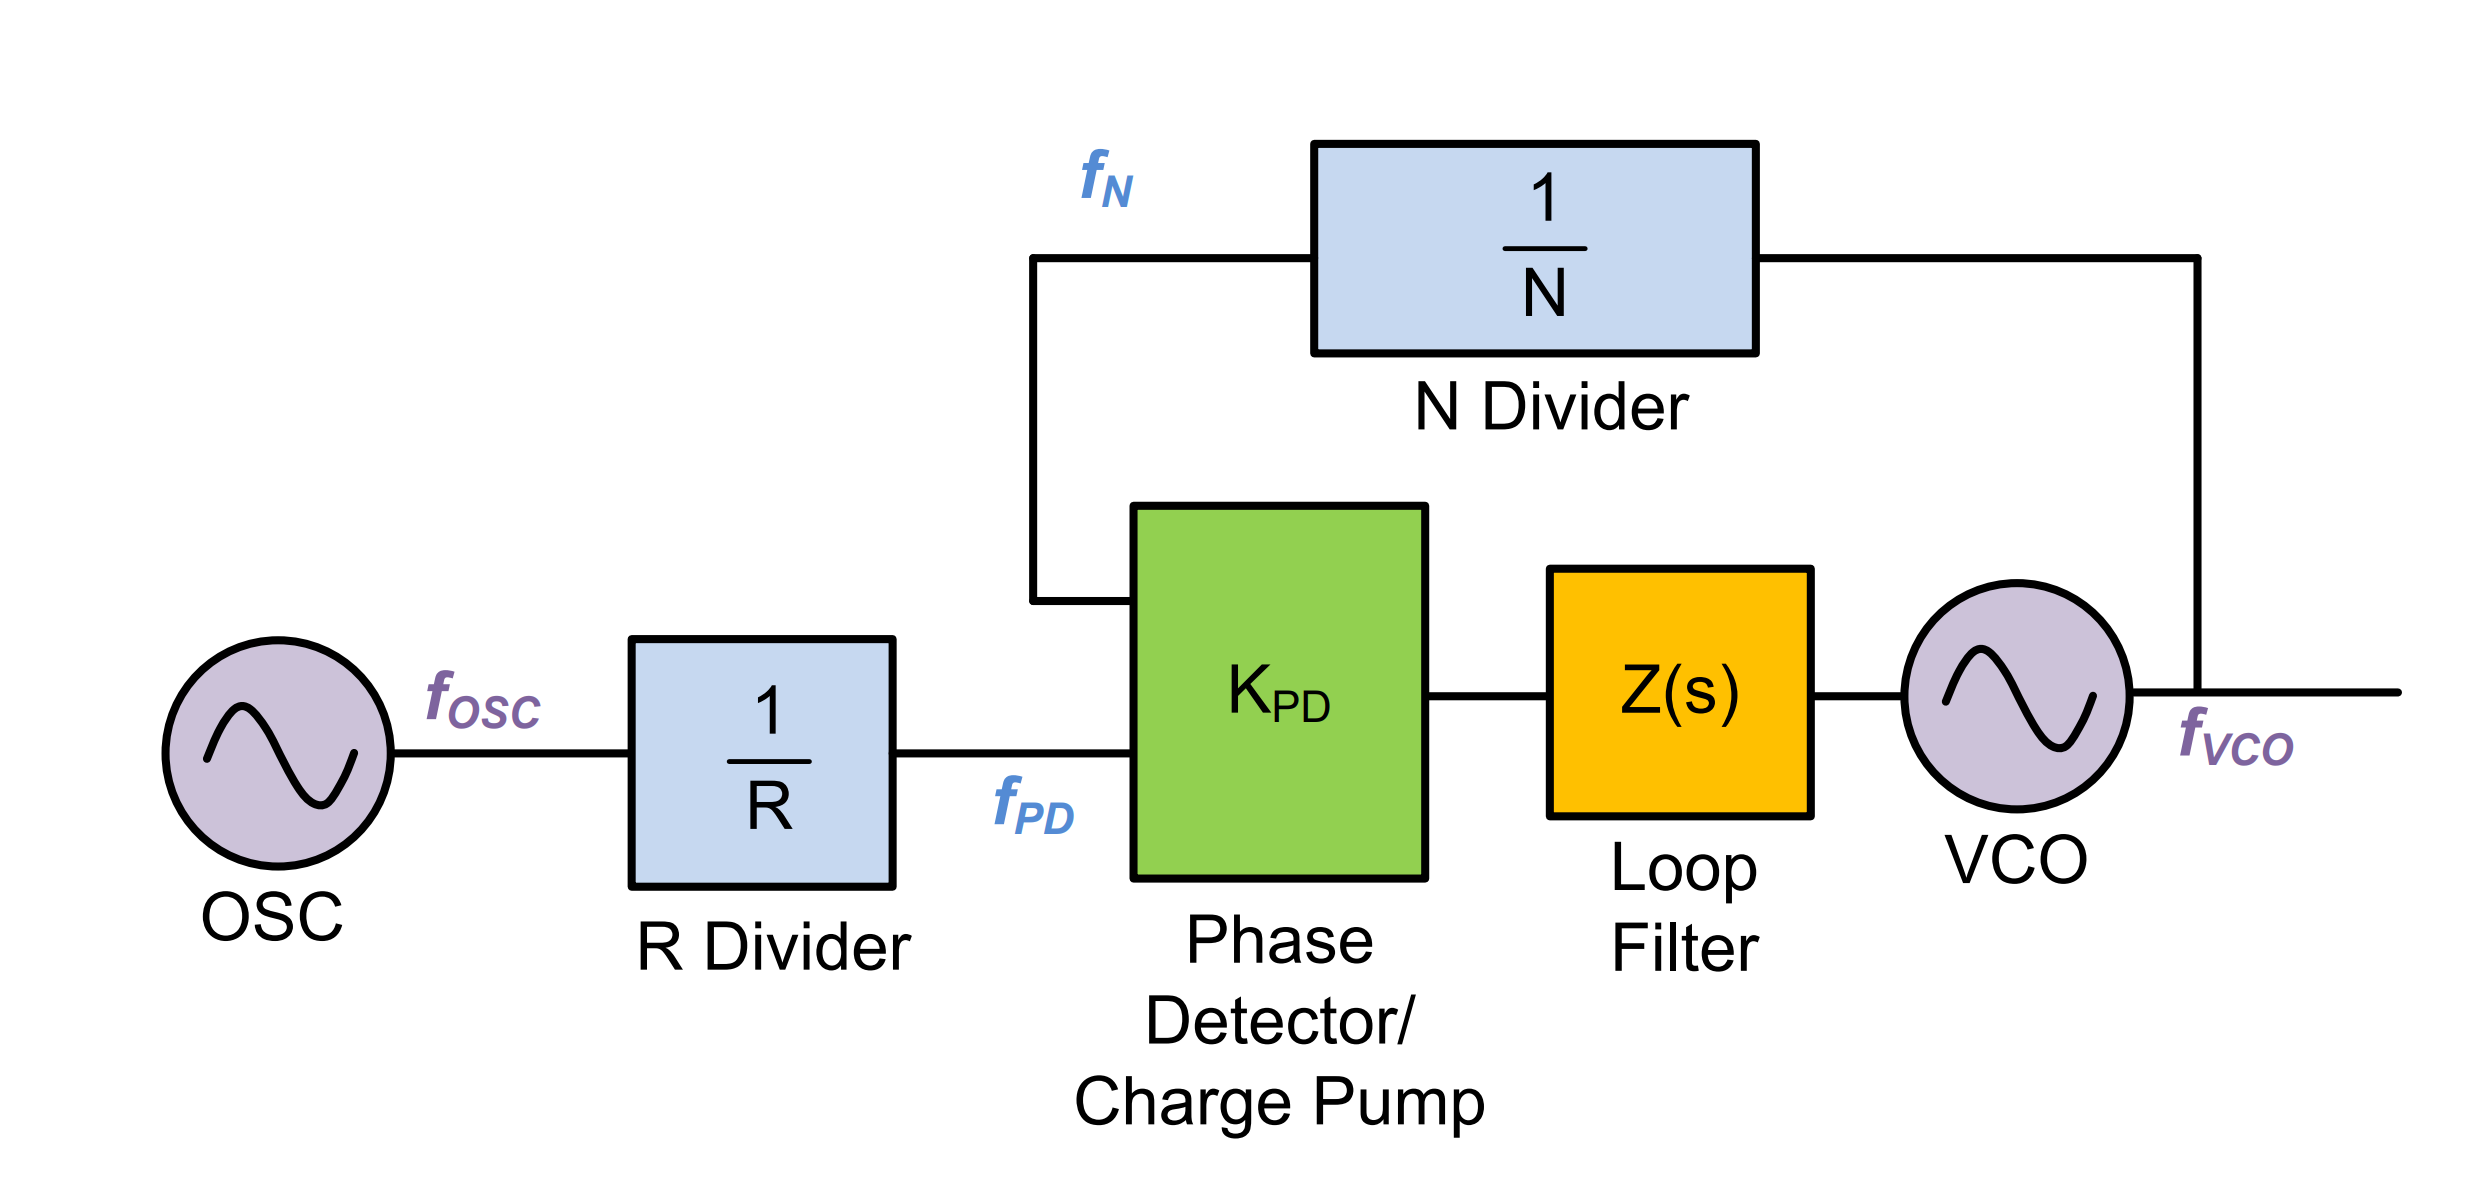
\includegraphics[width = \textwidth]{chap/04-work/img/pll_block}
	\caption[PLL block diagram]{General block diagram of a \gls{pll}}
	\label{fig:pll_block}
\end{figure}


\begin{table}[tbh]
	\caption[LMX2594 Filter characteristics]{Filter characteristics}
	\label{tab:lmx2594_filter}
	\centering
	\begin{tabularx}{\textwidth}{Xl}
		\toprule
		\textbf{Parameter}                         & \textbf{Value}             \\ \bottomrule
		VCO Gain                                   & \SI{239}{\MHz\per\volt}    \\
		Loop Bandwidth                             & \SI{32.7}{\kHz}            \\
		Phase Margin                               & \ang{69}                   \\
		Effective Charge Pump Gain                 & \SI{3}{\milli\ampere}      \\
		Phase Detector Frequency                   & \SI{24.576}{\MHz}          \\
		VCXO Frequency                             & Designed for \SI{15}{\GHz} \\
		[0.3cm]
		 \textbf{Loop filter components} &                            \\
		$C_{1,\text{LF}}$                          & \SI{2200}{\pico\farad}     \\
		$C_{2,\text{LF}}$                          & \SI{180}{\nano\farad}      \\
		$C_{3,\text{LF}}$                          & \SI{1800}{\pico\farad}     \\
		$R_{2}$                                    & \SI{160}{\ohm}             \\
		$R_{3,\text{LF}}$                          & \SI{180}{\ohm}             \\ \bottomrule
	\end{tabularx}
\end{table}

%todo deg

\begin{figure}[tbh]
	\centering
	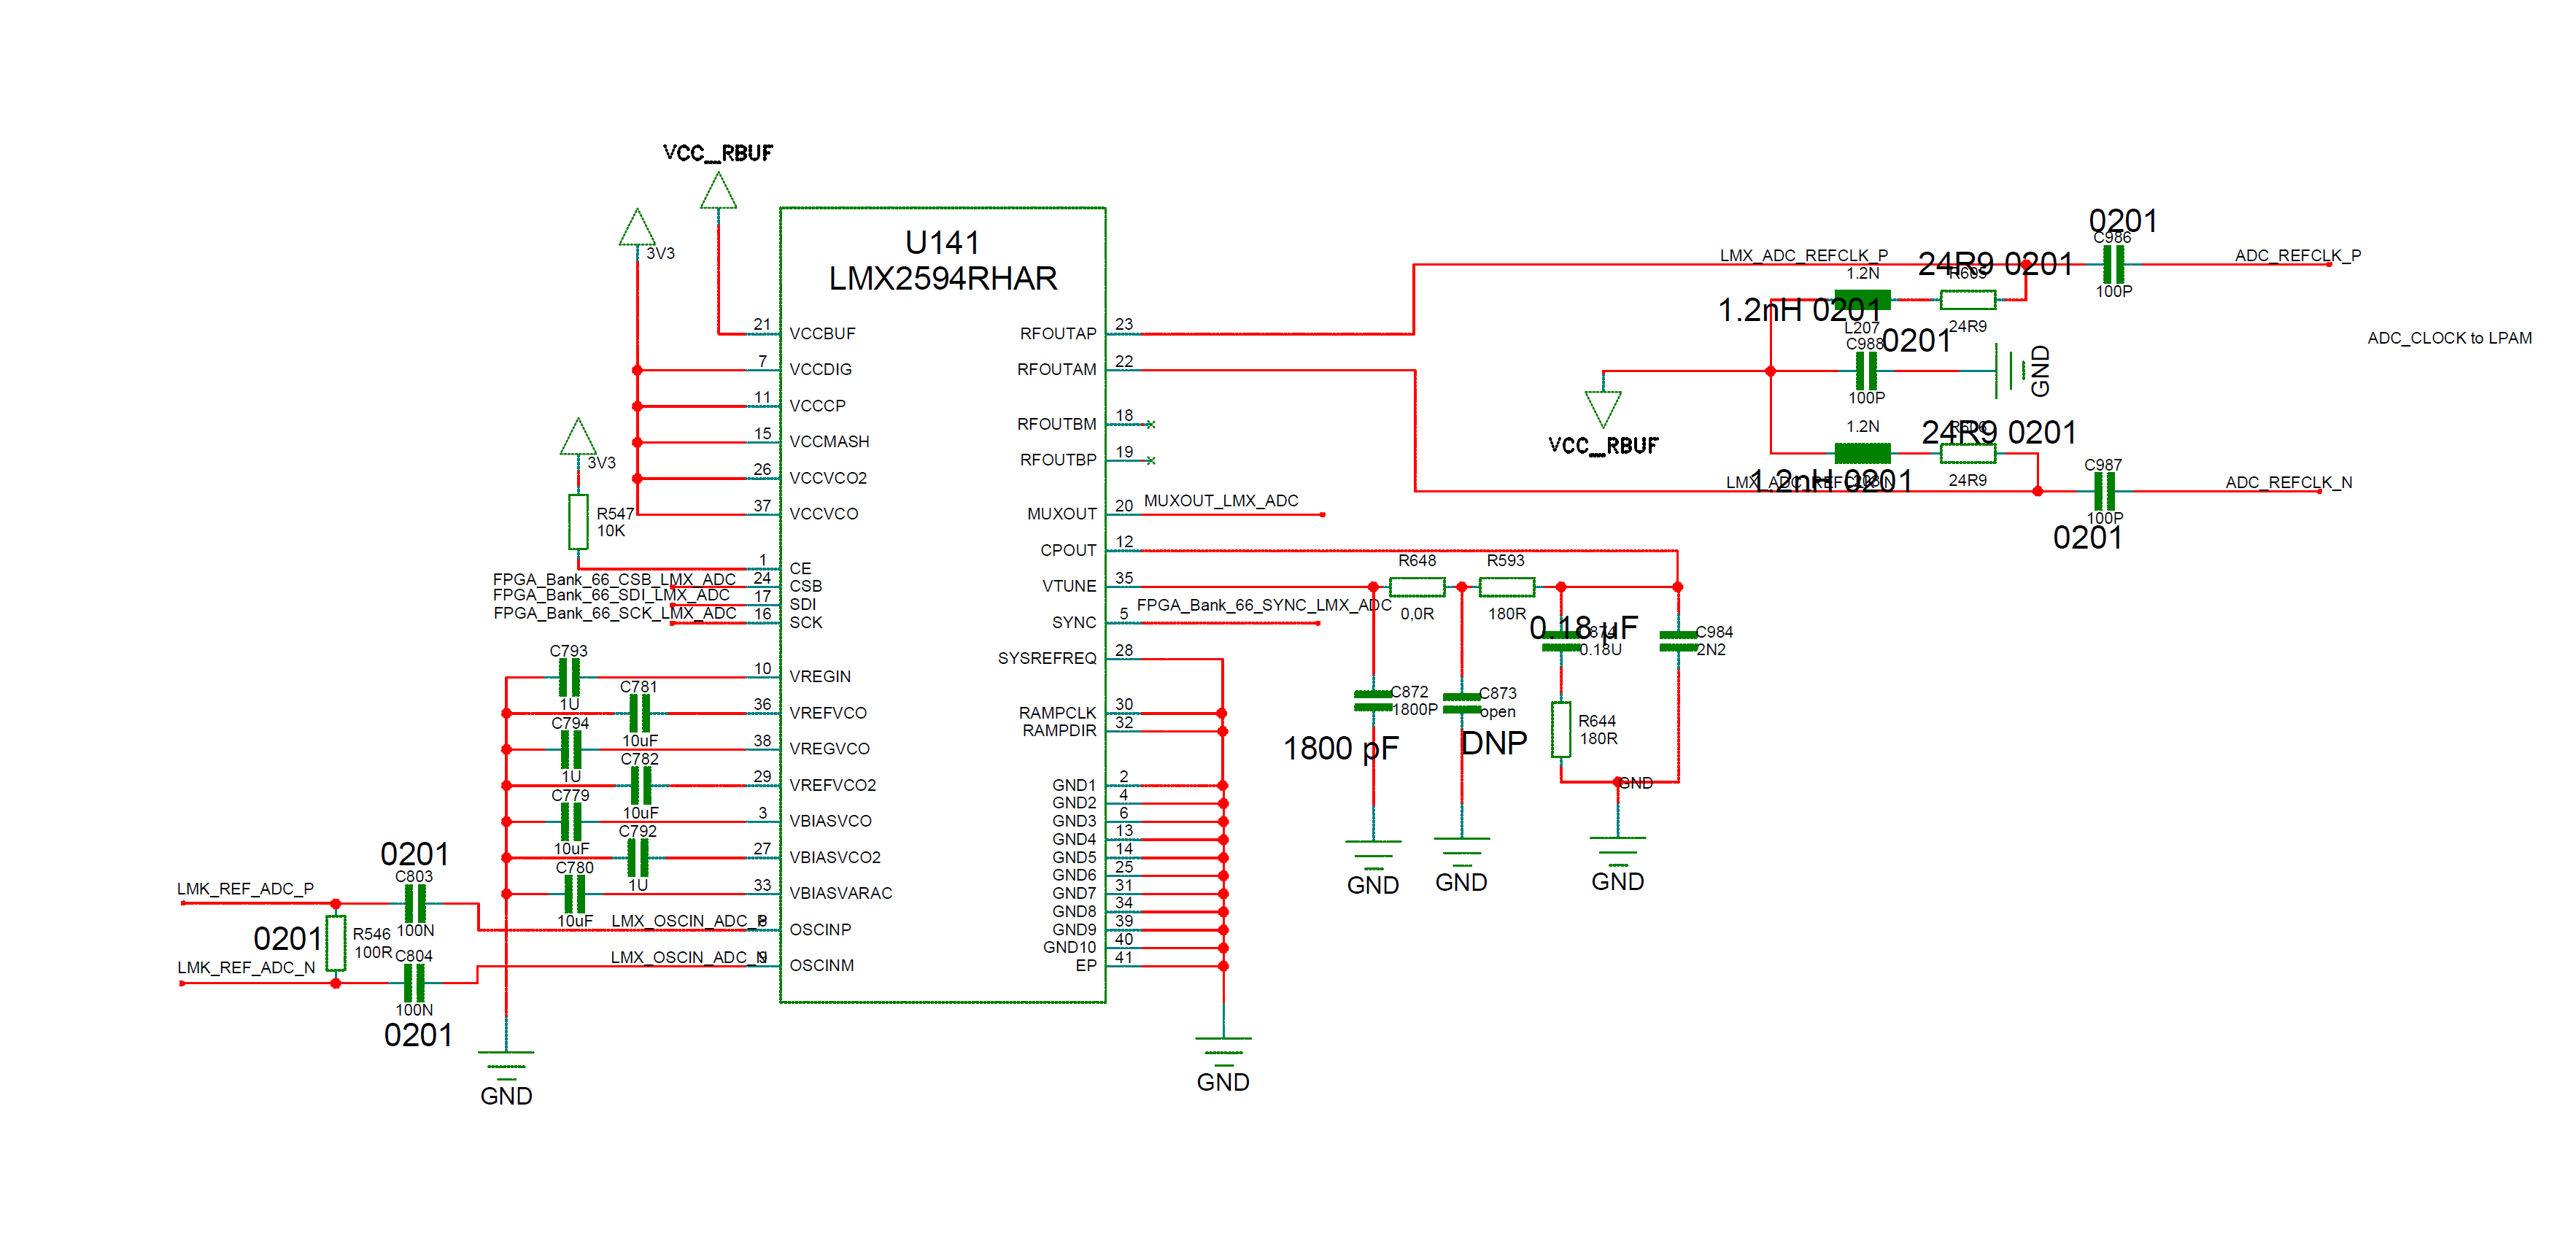
\includegraphics[width = \textwidth]{chap/04-work/img/lmx2594}
	\caption{Schematics of the LMX2594}
	\label{fig:lmx2594}
\end{figure}

\textbf{TODO}: Explain with help of timing diagram, why ADCs need to be at different PLLs -> outputs not individually programmable. phase difference between clocks needs to be 180° -> like two times interleaving

The necessary step size for the delay chips, when using 16 ADC@\SI{2}{\giga \sample \per \second} in time-interleaving mode, is: $\frac{\SI{2}{\giga \sample \per \second}}{16} = \SI{31}{\pico \second}$
However, providing individual clocks to the ADCs is not possible on the ZCU216 card. ADCs are grouped together into tiles, each tile containing four converters. One single reference clock signal is propagated to all tiles. Sampling clock is adjusted at each tile individually, however this clocking signal is the same for all of the four converters in the tile. Normally, only one reference clock can be provided. Analyzing the schematic of the zcu216 board revealed however, that there are pins leading to the FPGA banks (224 to 227), labeled as clocks for the individual tiles. Two of the clocks are not connected (224 and 227). 225 is provided via SMA cable, the other comes from the LPAM clock connector.  

Clock to THA: \SI{500}{\mega \hertz}

Total Hold time: \SI{1}{\nano \second}

$\rightarrow$ Step size for delay:
\begin{equation}
	\frac{\SI{1}{\nano \second}}{16 \, \text{channels}} = \SI{62.5}{\pico \second}
\end{equation}

Aperture delay, jitter, need to be taken into account to determine the max. sampling frequency.
\begin{figure}[tbh]
	\centering
	\tikzexternaldisable
	\begin{tikztimingtable}
		TH1 & 1L 8H N(A1) 8H 16L \\
		TH2 & 2L 16H 15L \\
		TH3 & 3L 16H 14L \\
		TH4 & 4L 5H N(B1) 11H 13L \\
		\\
		TH5 & 5L 8H N(A2) 8H 12L \\
		TH6 & 6L 16H 11L \\
		TH7 & 7L 16H 10L \\
		TH8 & 8L 5H N(B2) 11H 9L \\
		\\
		TH9 & 9L 8H N(A3) 8H 8L \\
		TH10 & 10L 16H 7L \\
		TH11 & 11L 16H 6L \\
		TH12 & 12L 5H N(B3) 11H 5L \\
		\\
		TH13 & 13L 8H N(A4) 8H 4L \\
		TH14 & 14L 16H 3L \\
		TH15 & 15L 16H 2L \\
		TH16 & 16L 5H N(B4) 11H 1L \\
		\extracode
		\tablerules
		\draw [dashed] (A1) --node[midway, anchor = west]{ADC1} (B1) ;
		\draw [dashed] (A2) --node[midway, anchor = west]{ADC2} (B2) ;
		\draw [dashed] (A3) --node[midway, anchor = west]{ADC1} (B3) ;
		\draw [dashed] (A4) --node[midway, anchor = west]{ADC2} (B4) ;
	\end{tikztimingtable}
	\tikzexternalenable
	\caption[Track-And-Hold Timing diagram]{\gls{tha} Timing diagram. Shows the clocking of the \gls{tha}, high level = HOLD, low level = TRACK. Dashed line represents the sampling of the \gls{adc}.}
	\label{fig:THA}
\end{figure}
%todo what does the dashed line show?


\subsection{Digital-To-Analog-Converter Balun Channel}
For test purposes, two \gls{dac} channels from the read-out card are routed on the sampling board.
In this way, test signals can be generated right on the read-out card, without the need for an external signal generator. 

\begin{figure}[tbh]
	\centering
	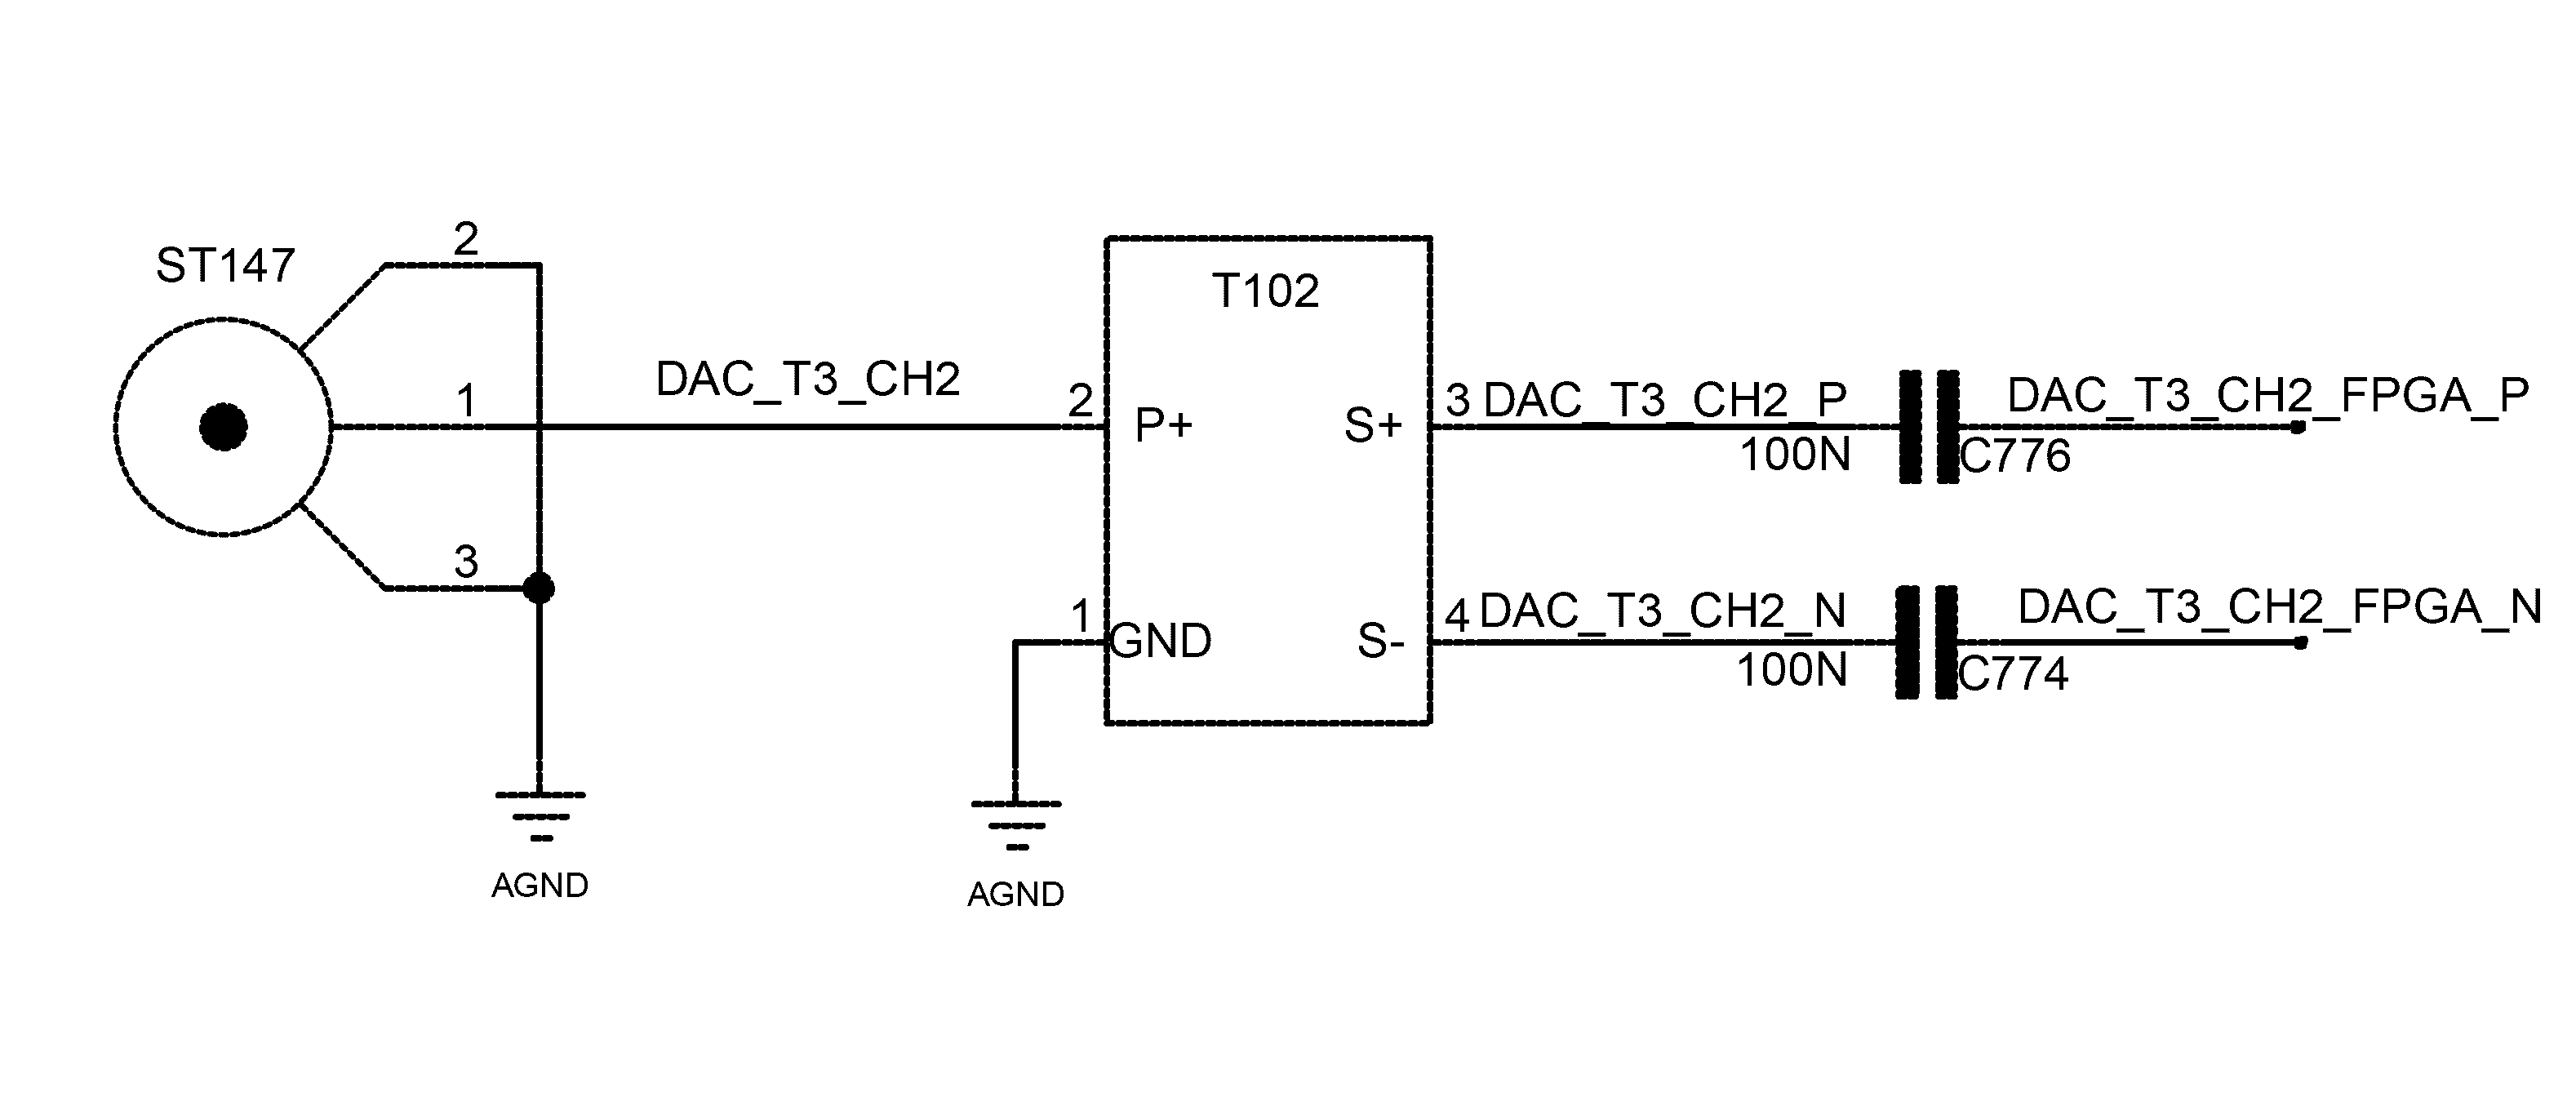
\includegraphics[width = \textwidth]{chap/04-work/img/dac_channel}
	\caption{DAC-channel with balun. Signal travels from right to left.}
	\label{fig:dac_channel}
\end{figure}


\subsection{Power Supply}
On the \gls{kapture} sampling board, the ADP1708 from \textit{Analog Devices} is used to provide a power supply for the \glspl{tha}. 
For the Track-And-Hold amplifiers a new power supply unit, the ADP1741 from \textit{Analog Devices}, should be used. It is necessary to think about the amount of power supply chips needed.
As a rule of thumb, the power supply should provide twice the maximum power needed by the components it drives. \cite{michele}
The power consumption/maximum current for the respective components on the sampling board is listed in \autoref{tab:kapturecomp}. 

It is necessary to think about the amount of power supply chips needed. As a rule of thumb, the power supply should provide twice the maximum power needed by the components it drives. \cite{michele} The power consumption/maximum current for the respective components on the sampling board is listed in \autoref{tab:kapturecomp}. 
\begin{table}[tbh]
	\caption{Power consumption of components on the board}
	\label{tab:kapturecomp}
	\begin{minipage}{\textwidth}
		\centering
		\begin{tabularx}{\textwidth}{Xlllll}
			\toprule
			\textbf{Component}          & $V_\text{cc}$ (V) & $I_\text{max}$ (A)                        & $P_\text{max}$ (W) & $\#_\text{parts}$ & $I_\text{tot}$\footnote{for 16 \glspl{adc}} (A) \\ \midrule
			HMC5649 \gls{tha}           & 2                 & 0.221                                     & 0.442              & 16                & 3.536                                           \\
			                            & -5                & -0.242                                    & 1.21               &                   & 3.872                                           \\
			HMC856 (Delay)              & -3.3              & 0.185                                     & -0.611             & 16                & 2.96                                            \\
			HMC987LP5E (Fan-Out buffer) & 3.3               & 0.234\footnote{All Outputs and RF-Buffer} & 0.772              & 2                 & 0.468                                           \\
			LMC0480 \gls{pll}           & 3.3               & 0.590\footnote{All CLKs}                  & 1.947              & 1                 & 0.590                                           \\
			VCXO                        & 3.3               & 0.03                                      & 0.198              & 1                 & 0.03                                            \\ \bottomrule
		\end{tabularx}
	\end{minipage}
\end{table}
%todo why two rows for the HMC THA. what are the upper/lower values?

The maximal current which the ADP1741 can provide @\SI{2}{\volt} is \SI{2}{\ampere}.
This means, with one \gls{tha} amplifier requiring a maximal current of \SI{0.221}{\ampere}, one ADP1741 can handle four units according to the rule mentioned beforehand ($I_{\text{max\_ADP1741}} = \SI{2}{\ampere} > 2 * I_\text{tot}, I_\text{tot} = 4 \cdot \SI{0.221}{\ampere} =  \SI{0.884}{\ampere}$).
%todo move to eq env?


\section{Layout}
%Both analog and digital signals require a wideband
%signal propagation and a low noise of both voltage and
%time levels. Therefore the PCB is made by ROGER 4003
%material and the signals are routed by dedicated
%transmission lines. Well separated analog and digital
%grounds in conjunction with ad-hoc RF filters located
%closer at the critical components have been adopted to
%reduce the influence of the digital circuit on the analog
%devices. Moreover, the via fences and guard ring
%techniques have been employed in the PCB layout in
%order to reduce the cross-talk between adjacent
%transmission lines, the electromagnetic interference (EMI)
%and improve the performance at high frequency [6]. A low
%time jitter is required, which is dependent on deterministic
%and Gaussian contributions. The deterministic jitter (DJ)
%depends on the duty cycle distortion, cross-talk, EMI, etc.
%This component has been drastically reduced by the
%techniques mentioned before regarding hardware layout
%techniques, moreover, the residual noise can be measured
%and corrected in the FPGA.


\subsection{PCB Structures Overview} \label{ssec:pcb_structs}
An overview over the basic structures on a \gls{pcb} is given.

\paragraph{Traces}
A \textit{trace} is a strip of metal, which establishes an electrical connection and carries signals between two (or more) points in the horizontal plane of a \gls{pcb}. \cite{xilDecouple}


\paragraph{Planes}
\textit{Plane} denotes an uninterrupted area of metal, which covers the whole \gls{pcb} layer. If this area only covers only part of the layer, it is called a \textit{planelet}. These areas provide power distribution across the \gls{pcb} and present an important transmission medium for the return current\footnote{Any current, which is injected into the components/boards, needs a return path, as otherwise there is no closed circuit.}. \cite{xilDecouple}

\paragraph{Vias}
A via is metal-plated hole, which is used to route a trace in vertical direction, i.e. from the \gls{pcb} outer layer to the inner layers. They carry signals and power. Three types of vias are \cite{vias}:
\begin{itemize}
	\item Blind via: A blind via connects the surface layers with at most three layers below.
	\item Buried via: A buried via only connects internal layers.
	\item Through via: A through via goes from one \gls{pcb} surface to another and is used to connect any layer. 
\end{itemize}
\begin{figure}[tbh]
	\centering
	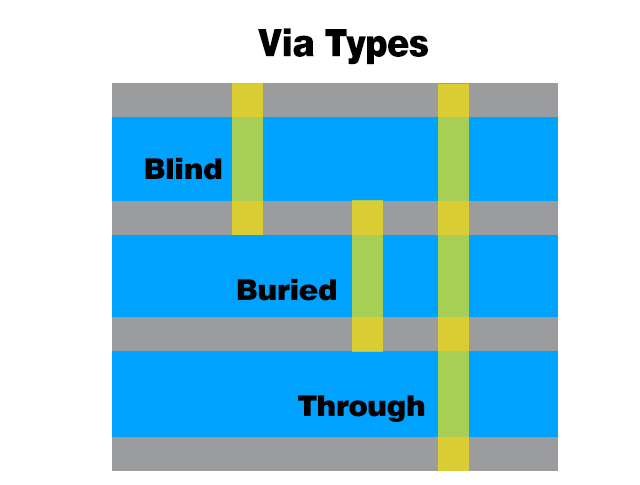
\includegraphics[width = 0.7\textwidth]{chap/04-work/img/vias}
	\caption[Via types]{Visualization of via types \cite{vias}}
	\label{fig:vias}
\end{figure}
\textbf{TODO:} 
	\begin{itemize}
		\item Via fences
		\item Pads
	\end{itemize}
%todo bild

In this design only blind and through vias are used.

\subsection{\gls{pcb} Substrate}
TODO
Megtron6 Laminate R-5775 Prepreg R-5670

$\epsilon_r = 3.61$ at \SI{10}{\giga \hertz}, $\epsilon_r = 3.71$ at \SI{1}{\giga \hertz}
\subsection{Floor Planning}
TODO
\subsection{Transmission lines}
TODO 

Transmission lines carry high-frequency signals, therefore the geometry of them is important, as this affects the impedance.
For single-ended the waveguide characteristic impedance should be \SI{50}{\ohm}, for differential signals \SI{100}{\ohm}.
For slow signals not that crucial, but for sensitive, high-speed signals, e.g. clocking signals, proper calculation is very important to ensure signal integrity and reduce reflection and damping. 

For \glspl{pcb} usually coplanar waveguides are used for signal propagation.
The characteristic impedance depends on the dielectric, the trace width, separation between traces and separation between the signal traces and the ground planes/traces.
Formulas to calculate the characteristic impedance are quite lengthy and not easy to solve.
Luckily, tools\footnote{which are quite expensive though, if a high variety of geometries is necessary} exist to quickly calculate the geometric values needed for appropriate impedance. %todo no lucky
For the design, the Si9000e \gls{pcb} field solver from \textit{Polar} (see \autoref{fig:polaris}) is used to calculate the necessary trace widths, separations, etc.

\begin{figure}[tbh]
	\centering
	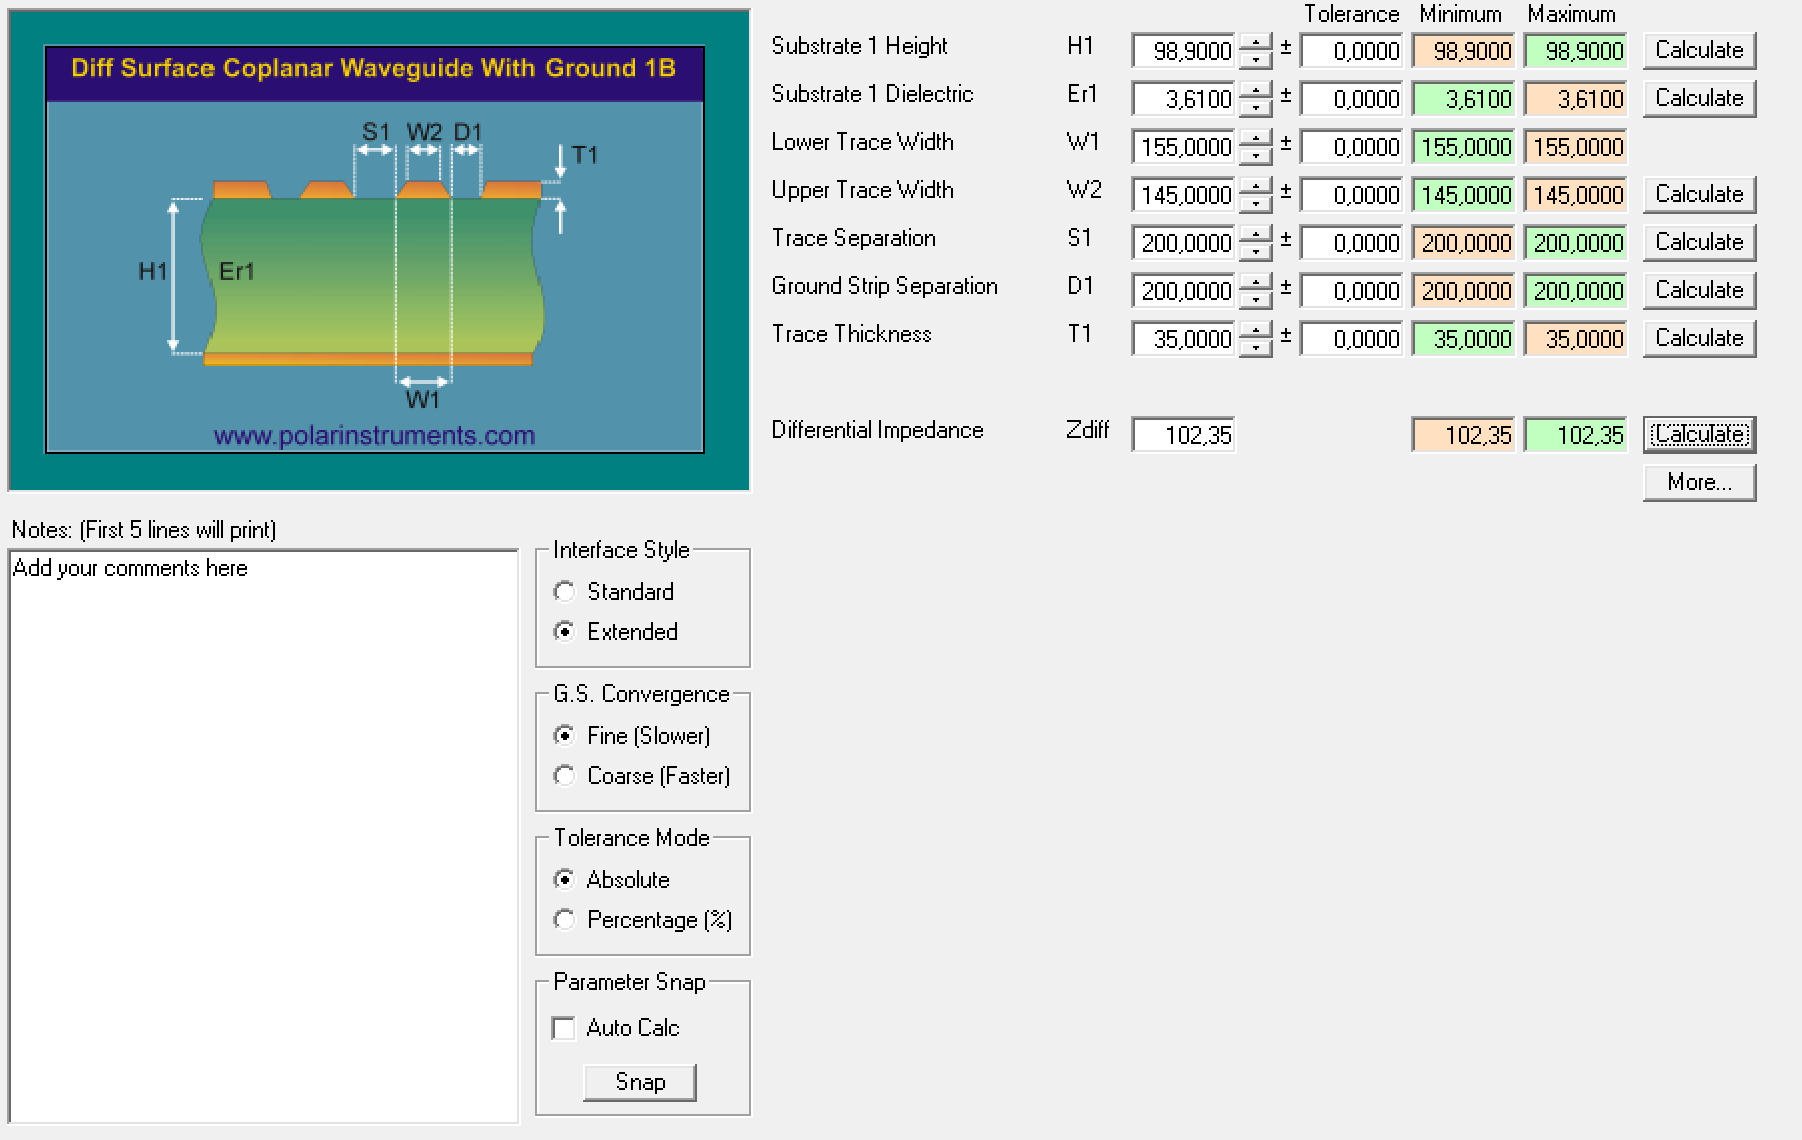
\includegraphics[width = \textwidth]{chap/04-work/img/polaris}
	\caption{Polaris Solver} %todo screenshot, .. showing, ...
	\label{fig:polaris}
\end{figure}

Three geometries of waveguides are used in this design which are described in the following.
Furthermore, geometric dimensions calculated with the Si9000e tool are presented.
In principle, the geometries can be taken from the design of the sampling card of \gls{kapture} system.
As the dielectric constant of the substrate is slightly different (\gls{kapture}: 3.52, here: 3.61), the impedance has to be recalculated to check whether the characteristic value impedance still lies in the \SI{10}{\percent} tolerance.

\paragraph{Surface Coplanar Waveguide with Ground}
The surface coplanar waveguide has the geometry shown in \autoref{fig:microstrip_geometry}.
The single trace of thickness $t$ and width $a$ lies between two ground planes on a dielectric of thickness $h$ and the effective dielectric constant $\epsilon_r$.
Another ground plane is located at the bottom of the dielectric.
Separation between trace and ground plane is defined as $(b-a)/2 := d$. 

\begin{figure}[!htbp]
	\centering
	\includegraphics[width = \textwidth]{chap/04-work/img/cw}
	\caption{Coplanar Waveguide with Ground}
	\label{fig:microstrip_geometry}
\end{figure}

Trace width is assumed to be $a = \SI{180}{\micro\meter}$.
In the tool, an upper and a lower trace width can be specified, therefore taking into account manufacturing processes. %todo whoch tool
As the exact upper trace width is not known, both are assumed to be \SI{180}{\micro\meter}.
Trace-To-Ground Separation, or "Ground Strip Separation", is defined by the manufacturing technology of the \gls{pcb} process: $d = \SI{250}{\micro\meter}$
With $h = \SI{98.9}{\micro \meter}$, $\epsilon_r = 3.61$ (at \SI{10}{\GHz}) this results in a characteristic impedance of \SI{52.90}{\ohm}. This lies well in the tolerance area. %todo of...

Over the frequency range, the value of the effective dielectric constant changes from 3.71 (at \SI{1}{\GHz}) to 3.61 (at \SI{10}{\GHz}).
As the tool provides the possibility to calculate the impedance versus a changing parameter, the influence of a changing dielectric was calculated. %todo which tool
As can be seen in \autoref{fig:surf_z0_vs_dk}, with higher effective dielectric constant, the characteristic impedance decreases (see \autoref{fig:surf_z0_vs_dk}).

The only parameters, which are not defined by the manufacturing process and therefore can be altered, are the ground strip separation and the trace width. %todo always restate the physical symbols defined earlier
When altering the trace width, the tool automatically assumes an upper trace width, which is \SI{25}{\micro \meter}.

\textbf{TODO}: fix plot. too big

\begin{figure}
	\centering
	\includegraphics[width = \textwidth]{chap/04-work/img/surf_z0_vs_dk.tikz}  
	\caption{Characteristic impedance $Z_o$ vs effective dielectric constant $\epsilon_r$ of a surface coplanar waveguide with ground}
	\label{fig:surf_z0_vs_dk}
\end{figure}


 \paragraph{Differential Pairs on Surface}
\begin{figure}[!htbp]
	\centering
	\includegraphics[width = \textwidth]{chap/04-work/img/eccw}
	\caption{Edge-Coupled Coplanar Waveguide}
	\label{fig:eccw_geometry}
\end{figure}

\paragraph{Differential Pairs between Layers}
\begin{figure}[!htbp]
	\centering
	\includegraphics[width = \textwidth]{chap/04-work/img/docw}
	\caption{Differential Offset Coplanar Waveguide}
	\label{fig:docw}
\end{figure}






\section{Production}
